%%%%%%%%%%%%%%%%%%%%%%%%%%%%%%%%%%%%%%%%%%%%%%%%%%%%%%%
%% Bachelor's & Master's Thesis Template             %%
%% Copyleft by Artur M. Brodzki & Piotr Woźniak      %%
%% Faculty of Electronics and Information Technology %%
%% Warsaw University of Technology, 2019-2020        %%
%%%%%%%%%%%%%%%%%%%%%%%%%%%%%%%%%%%%%%%%%%%%%%%%%%%%%%%

\documentclass[
    left=2.5cm,         % Sadly, generic margin parameter
    right=2.5cm,        % doesnt't work, as it is
    top=2.5cm,          % superseded by more specific
    bottom=3cm,         % left...bottom parameters.
    bindingoffset=6mm,  % Optional binding offset.
    nohyphenation=false % You may turn off hyphenation, if don't like.
]{eiti/eiti-thesis}

\langpol % Dla języka angielskiego mamy \langeng
\graphicspath{{img/}}             % Katalog z obrazkami.
\addbibresource{bibliografia.bib} % Plik .bib z bibliografią

\begin{document}

%--------------------------------------
% Strona tytułowa
%--------------------------------------
\EngineerThesis % Dla pracy inżynierskiej mamy \EngineerThesis
\instytut{Informatyki}
\kierunek{Informatyka}
\specjalnosc{Inżynieria systemów informatycznych}
\title{
    Zastosowanie analizy obrazu twarzy do sterowania aplikacją na urządzeniach z systemem Android 
}
\engtitle{ % Tytuł po angielsku do angielskiego streszczenia
    Facial image based application control on Android devices
}
\author{Adamski Maciej}
\album{300184}
\promotor{prof. dr hab. inż. Przemysław Rokita}
\date{\the\year}
\maketitle

%--------------------------------------
% Streszczenie po polsku
%--------------------------------------

 \cleardoublepage % Zaczynamy od nieparzystej strony
 \streszczenie
 
 Celem pracy inżynierskiej było stworzenie aplikacji na urządzenia z systemem \textit{Android}, która przy pomocy analizy twarzy będzie reagowała na gesty użytkownika takie jak mruganie czy ruch gałkami ocznymi.
 
 \par
 
 Został przygotowany zestaw algorytmów do~detekcji poszczególnych fragmentów twarzy, które następnie były testowane pod kątem skuteczności detekcji i~złożoności czasowej. Do~implementacji wybranych metod przetwarzania obrazu zostały użyte biblioteki \textit{OpenCV} oraz \textit{Dlib}.
 Najlepsze rozwiązania z~poszczególnych grup zostały wykorzystane w finalnym projekcie oprogramowania. Proces detekcji twarzy odbywa się przy pomocy algorytmu opartego na~\textit{Histogramach zorientowanych gradientów}, natomiast znaczniki są~wykrywane dzięki metodzie \textit{Kazemi}. \textit{Punkty charakterystyczne twarzy} pozwalają określić położenie na~zdjęciu oczu, a~także stwierdzić czy są one zamknięte przy użyciu współczynnika \textit{Eye Aspect Ratio}. Wykorzystywane jest \textit{progowanie na~podstawie dystrybuanty} celem wyznaczenia środka źrenicy.
 
 \par
 
 Końcowym efektem pracy dyplomowej jest prosta aplikacja, która prezentuje działanie analizy obrazu oraz reaguje na~ruch oczami w~poziomie czy mruganie użytkownika. Wykrycie takich gestów przedstawione było w~zrozumiałej formie przez wyświetlanie komunikatów oraz przesuwanie obrazów w prostej galerii zdjęć. 
 
 \par
 
 Praca pomogła zapoznać się z~wytwarzaniem oprogramowania użytkowego na systemy Android. Przyniosła również dużo wiedzy z~zakresu przetwarzania obrazu oraz sieci neuronowych i~uczenia maszynowego. Pozwoliła też poznać dwie popularne biblioteki z~dziedziny widzenia komputerowego. 

 \slowakluczowe Cyfrowe przetwarzanie i analiza obrazów, Detekcja twarzy, Śledzenie oczu, Programowanie aplikacji mobilnych, Kontrola aplikacji z wykorzystaniem obrazów

%--------------------------------------
% Streszczenie po angielsku
%--------------------------------------

 \newpage
 \abstract

The main goal of this thesis was to create the application for the devices that run the Android operating system, which with the aid of face analysis, would be able to react to the user gestures such as blinking or eyeball movement.

\par

To detect specific parts of the face there was prepared a set of algorithms. Each of them was further tested in terms of detection effectiveness and time complexity. The chosen image processing methods were implemented with the usage of \textit{OpenCV} and \textit{Dlib} libraries. The best solutions from each group were used in a final software project. The face detection process is performed with the aid of an algorithm based on a \textit{Histogram of Oriented Gradients}, whereas the facemarks are being detected with the \textit{Kazemi} method. The face pointers allow determining the eyes' location on the photo as well as ascertain whether they are closed with the \textit{Eye Aspect Ratio} coefficient. There is used the \textit{thresholding by cumulative distribution function} in order to find the center of the pupil.

\par

The final result of this thesis is a simple application that presents the working of the image analysis, reacts to horizontal eyeballs movement, and to blinking. Those gestures detection were shown to the user in a readable way as a notification and also in the form of moving images in the simple photo gallery.

\par

This work was a helpful introduction to application development on Android devices. It also brought a significant amount of knowledge related to image processing, neural networks, and machine learning. Moreover, it allowed getting to know the two popular libraries from the domain of computer vision.


 \keywords Digital image processing and analysis, Face detection, Eye gaze tracking, Mobile application development, Image based application

%--------------------------------------
% Oświadczenie o autorstwie
%--------------------------------------
\cleardoublepage  % Zaczynamy od nieparzystej strony
\pagestyle{plain}
\makeauthorship

%--------------------------------------
% Spis treści
%--------------------------------------
\cleardoublepage % Zaczynamy od nieparzystej strony
\tableofcontents

%--------------------------------------
% Rozdziały
%--------------------------------------
\cleardoublepage % Zaczynamy od nieparzystej strony
\pagestyle{headings}

\newpage

\section{Wstęp}


\subsection{Cel pracy}

Celem niniejszej pracy dyplomowej było zaprojektowanie i~implementacja aplikacji na~urządzenia z systemem Android, która wykorzystując analizę twarzy miała reagować na~gesty użytkownika. By~to~osiągnąć należało zaimplementować i~przetestować wybrane metody przetwarzania obrazów do detekcji twarzy i~wybranych jej fragmentów. Następnie, na~podstawie wyników testów wybrać najlepsze, które miały zostać wykorzystane do~sterowania prostą aplikacją w systemie Android prezentującą działanie detektorów i~ich przykładowe zastosowanie.



\subsection{Motywacja pracy}

W~dzisiejszych czasach coraz większą popularność zyskuje wirtualna rzeczywistość, bezdotykowa obsługa urządzeń czy dostosowanie interfejsu aplikacji do~osób niepełnosprawnych. Rozwiązania niegdyś znane wyłącznie z~filmów, które wydawały się niemożliwe do~stworzenia nie są już pieśnią przyszłości.

\par

Dla ludzi o~różnych nieprawidłowościach ruchowych kończyn górnych użytkowanie w~codziennym życiu takich urządzeń jak komputer czy telefon prawdopodobnie jest problematyczne. Zapewnienie im~możliwości sterowania interfejsami tych narzędzi za~pomocą gestów np. twarzy lub komendami głosowymi może być pożądaną przez nich alternatywą. 

\par

W dziedzinie sterowania głosem istnieją bardzo dobrze rozwinięte systemy takie jak Siri, Alexa czy asystent Google. Powszechne stosowane są w~urządzeniach przenośnych i~systemach inteligentnego domu. Natomiast analiza obrazu i~gestów nie jest już tak szeroko rozpowszechniona, a~również niesie duże możliwości w aspekcie bezdotykowego sterowania urządzeniami.  

\par

Zostało stworzonych już wiele gier wykorzystujących wirtualną rzeczywistość, w~której kamera podąża za~ruchami głowy gracza, a~interakcja ze światem gry wykonywana jest przez gesty rękami. Konstruktorzy takich rozwiązań cały czas dążą do jeszcze większej immersyjności. Wykorzystanie emocji czy analizy twarzy gracza pozwoliłaby mu się mocniej zanurzyć w~świat wirtualny, a~granica między rzeczywistością jeszcze bardziej by~się zacierała. 

\par

Czytanie artykułów czy przeglądanie galerii zdjęć na urządzeniu mobilnym wymaga ciągłych ruchów palcem po~ekranie. Byłoby wielkim uproszczeniem jakby tekst pisany przesuwał się automatycznie wraz ze~zmianą położenia oczu w czasie czytania kolejnych linii. 


\subsection{Etapy pracy}

Pierwszym etapem pracy nad projektem był przegląd znanych algorytmów oraz bibliotek mając na uwadze następujące zastosowania:

\begin{itemize}
    \item detekcja twarzy
    \item detekcja oczu
    \item detekcja źrenic
    \item detekcja punktów charakterystycznych twarzy
\end{itemize}

Wybór rozwiązań był nie tylko zależny od ich zalet typowo funkcjonalnych (skuteczność, szybkość itp.), ale także od~tego jak problematyczna jest integracja z~docelowym środowiskiem, jakości dokumentacji czy popularności w społeczności programistów.

\par

Następnie należało przetestować i~porównać ze sobą algorytmy w~odpowiednio podzielnych grupach. Zbierane były dane o~ich skuteczności oraz szybkości działania. Badania były prowadzone z~użyciem zbioru zdjęć, a~także na podstawie obrazu na~żywo z~kamery. Drugi przypadek miał bardzo istotny wpływ na~końcowy dobór algorytmów, ponieważ projekt z~założenia miał działać w~czasie rzeczywistym na~urządzeniach mobilnych. Na podstawie tak przeprowadzonych testów z~każdej grupy wybierana była jedna z~metod, która później była wykorzystywana w~finalnej wersji projektu.

\par

Następnym etapem było stworzenie aplikacji wykorzystującej przygotowany zestaw algorytmów. Demonstruje ona zarówno ich przykładowe zastosowanie w~kontekście sterowania interfejsem programu, ale także prezentuje na żywo analizę twarzy oraz pozwala wykonać opisane badania na~zestawie zdjęć.

\par

Końcowo, celem weryfikacji prawidłowego działania projektu przetestowano gotową aplikację w różnych warunkach codziennego użytkowania urządzenia.
\newpage

\section{Stos technologiczny} \label{section:tech_stack}

\subsection{System operacyjny Android}

Docelowym systemem operacyjnym, na który przygotowywany był projekt jest Android. Opiera się on na~jądrze Linux przystosowanym do~urządzeń mobilnych. Aktualnie stosowany jest też w~wielu innych urządzeniach elektronicznych takich jak telewizory, systemy audi czy nawet komputery pokładowe w samochodach.  

\subsection{Biblioteki}

\subsubsection{OpenCV}

Otwarta biblioteka widzenia komputerowego (ang. Open Source Computer Vision Library) \cite{opencv} - jedna z~najbardziej rozpowszechnionych bibliotek służąca do~przetwarzania obrazu i~widzenia komputerowego. Napisana z~użyciem języka C/C++ co zapewnia jej szybkie działanie i~możliwość wykorzystania niskopoziomowych mechanizmów. Z rozwiązań tego pakietu można korzystać na wielu systemach operacyjnych, a~dzięki wiązaniom do popularnych języków, kod może być pisany również w Javie czy Pythonie. Dzięki zastosowaniu takich mechanizmów sprzętowych jak CUDA \cite{nvidia_cuda} część obliczeń jest przenoszona z~jednostek arytmetycznych na akceleratory graficzne.


\subsubsection{OpenCV-contrib} \label{section:opencv_contrib}

Zbiorcza nazwa dla dodatkowych modułów \cite{opencv_contrib} biblioteki OpenCV. Nie są one zawarte w~wersji stabilnej API głównej pakietu. Jednak są to rozwiązania, które po szeregu testów i~pewnym okresie przejściowym mogą zostać włączone do podstawowego modułu. Znajdują się tam rozwiązania do~rozpoznawania twarzy \cite{opencvcontribface}, sieci konwolucyjnych czy detekcji obiektów. 

\subsubsection{Dlib}

Wieloplatformowy zestaw narzędzi \cite{dlib} napisany z~wykorzystaniem języka C++. Początkowo głównym obszarem zastosowań było uczenie maszynowe, lecz z~czasem zaczęto rozwijać także sektor sieciowy, przetwarzania obrazów czy operacje numeryczne. Rozpowszechniona jest na~licencji otwartego oprogramowania i~stale rozwijana. 

\subsubsection{CameraX}

Jeden z modułów \cite{camerax} tzw.~\textit{Android Jetpack} \cite{android_jetpack}. Biblioteka pozwalająca na~łatwą obsługę kamer zamontowanych w urządzeniu, na~którym uruchamiany jest program. Pozwala na przechwytywanie na~żywo obrazu, a~następnie jego analizę klatka po klatce oraz zapisywanie uzyskanego nagrania wideo i~zdjęć. 


\subsection{Języki programowania}

W projekcie wykorzystywane są dwa języki programowania:

\begin{itemize}
    \item Java - większość projektu napisane jest w tym języku
    \item C++ - wykorzystywany do wołania metod biblioteki Dlib przy pomocy JNI (rozdz. \ref{section:jni})
\end{itemize}

Dodatkowo, szablony aplikacji Android napisane są z~użyciem języka znaczników XML.

\subsection{JNI} \label{section:jni}

Natywny interfejs programistyczny dla języka Java (ang. Java Native Interface) \cite{jni} -  jest to~interfejs pozwalający uruchamiać natywne programy i~biblioteki w innym języku i~przeznaczone na inne systemy w~wirtualnej maszynie Java. W~projekcie pracy dyplomowej pozwala to~wykorzystać bibliotekę Dlib, która nie posiada gotowych wiązań do Javy. W~tym przypadku kod wywołujący metody tego pakietu jest napisany w~języku C++, który następnie wywoływany jest przez obiekty natywne w~maszynie wirtualnej. 
\newpage 

\section{Sposób badania algorytmów}

Algorytmy były badane i porównywane przy pomocy zestawu statycznych zdjęć z przygotowanego zbioru danych, jak i wykorzystując obraz na żywo z przedniej kamery urządzenia. Zbierane były dane na temat skuteczności i szybkości działania poszczególnych metod.

\subsection{Zbiór danych} \label{section:dataset}

Na potrzeby badań i porównania algorytmów przygotowany został zbiór danych składający się~z~80 zdjęć zawierających twarze. 

\par

Źródła zdjęć:

\begin{itemize}
    \item 50 zdjęć wybranych z datasetu \textit{Young and Old Images Dataset} \cite{young_old_dataset}
    \item 30 zdjęć wykonanych przez autora pracy dyplomowej
\end{itemize}

Zostały on dobrane w taki sposób, żeby zawierał zróżnicowane zdjęcia pod~wieloma względami, takimi jak: jakość obrazu, oświetlenie, powierzchnia zajmowana przez twarz, kolorystyka, płeć, kolor skóry, częściowe zakrycie twarzy, okulary czy odwrócona w bok głowa. 

\par

Wszystkie 80 zdjęć zostało opisanych ręcznie przez autora projektu na potrzeby badań, w~szczególności: obszar twarzy, oczu czy środek źrenic. 

\par

\subsection{Urządzenie do testów}

Wszystkie testy zostały przeprowadzone na urządzeniu Huawei P30 Pro w normalnym trybie wydajności i bez włączonego oszczędzania energii. 

\newpage

\section{Detekcja twarzy} \label{section:face_detection}

W~przetwarzaniu cyfrowym obrazu stosujemy technikę od ogółu do szczegółu. Przykładowo chcąc uzyskać barwę nadwodzia najpierw musimy wykryć samochód itp. W~pracy dyplomowej by~uzyskać dane dotyczące oczy czy znaczników potrzebujemy najpierw informacji o~tym czy twarz występuje na zdjęciu i~ewentualnie gdzie się ona na~nim znajduje. Dlatego pierwszym etapem przetwarzania na~potrzeby projektu jest detekcja ludzkiej twarzy. Z~dostarczonego obrazu uzyskujemy informację o~jej położeniu, a~w~następnych etapach możemy operować tylko na wycinku zdjęcia. 

\subsection{Algorytmy detekcji twarzy}

Na~potrzeby projektu zostało zaimplementowane użycie pięciu algorytmów, których celem jest wykrycie twarzy na zdjęciu. Krótki opis poszczególnych metod znajduje się w~następnych podrozdziałach.

\subsubsection{Klasyfikator kaskadowy} \label{section:face_casacde_classifier}
\textit{Cascade Classifier} to~jedno z podejść do~zadania klasyfikacji obiektów. Kaskadowość tego rozwiązania przejawia się tym, że składa się on z~łańcucha mniejszych klasyfikatorów. Z~danych wejściowych jednego mogą korzystać następne jako dodatkowe źródło informacji i~użyć je do własnej klasyfikacji. Z~tego powodu kolejne elementy są bardziej zaawansowane i~operują na większym zestawie danych. Dzięki swojej kaskadowej naturze modele takie mogą być lepiej trenowane i~dawać lepsze rezultaty niż klasyfikatory typu monolit.

\vspace{5mm}

Do ładowania i~przetwarzania kaskadowych klasyfikatorów w~projekcie używany jest moduł \textit{CascadeClassifier} \cite{cascade_opencv} biblioteki OpenCV. 

\paragraph{Haar}

Jednym z najbardziej znanych modeli klasyfikacji kaskadowej jest \textit{Haar}, który został opisany po~raz pierwszy w~2001 roku \cite{haar_proceeding}. Może on być używany do~klasyfikacji różnych obiektów, ale~autorzy skupiali się głównie na detekcji twarzy. Algorytm \cite{haar_towards} \cite{haar_pyimage} \cite{OBUKHOV2011517} bazuje na~podzieleniu zdjęcia na~regiony i~wykorzystaniu w~każdym z~nich pięciu cech krawędzi (\hyperref[{fig:haar_features}]{rys.~\ref{fig:haar_features}}). Algorytm porównując jasność pikseli w~białej i~czarnej części stwierdza czy istnieją krawędzie lub linie. Cechy składające się tylko z~dwóch regionów odpowiadają za~wykrycie pionowych i~poziomych krawędzi. Zestaw trzech za~detekcje linii. Natomiast kwadratowa cecha za~zmiany przekątne. W~dzisiejszych czasach Haar nie jest już tak często stosowany jak jeszcze parę lat temu.

\begin{figure}[!h]
    \begin{center}
        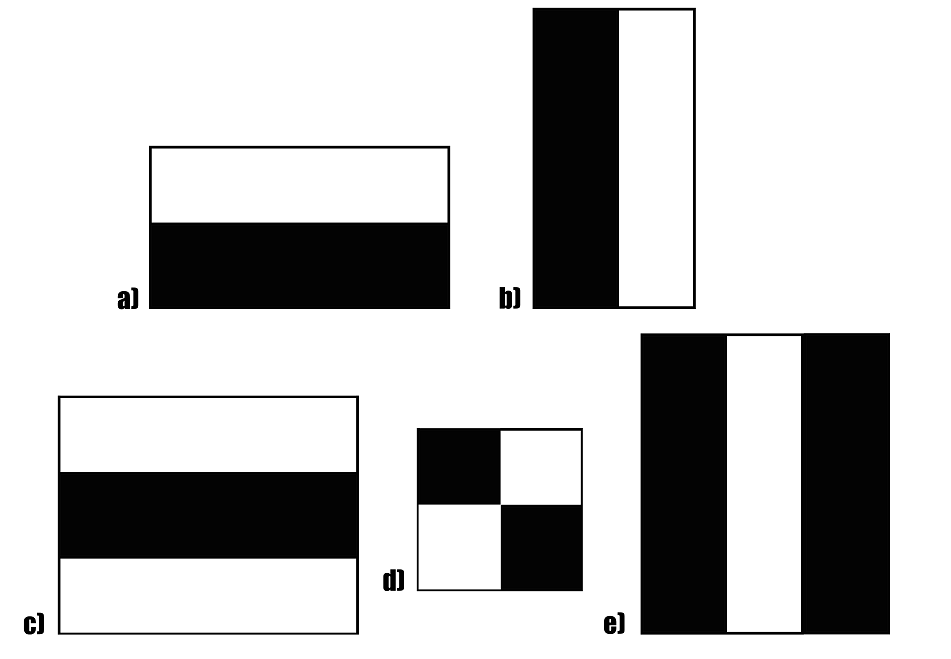
\includegraphics[scale=0.2]{img/face_section/haar_features.png}
        \caption{Cechy krawędzi modelu Haar. Źródło: \cite{haar_towards}}
        \label{fig:haar_features}
    \end{center}
\end{figure}

Na potrzeby pracy dyplomowej wykorzystywany jest model \textit{Haarcascade Frontalface Default} \cite{haar_frontal} autorstwa Rainera Lienharta.



\paragraph{Local binary patterns}
Metoda ta porównuje piksele z~ośmioma swoimi najbliższymi sąsiadami w~ustalonej kolejności. Jeśli jasność głównego piksela jest większa niż porównywanego to~na~odpowiedniej pozycji 8-bitowego ciągu wstawiana jest wartość~1, inaczej~0. Następnie z~uzyskanych w ten sposób liczb tworzony jest histogram używany jako deskryptor cech. Takie dane mogą być użyte do uczenia maszynowego. \cite{comp_haar_lbp}

\par

Jest to metoda cechująca się wysoką szybkością działania i~z~tego powodu stosowana w systemach z~ograniczonymi zasobami sprzętowymi. Niestety kosztem efektywności.

\par

W projekcie stosowany jest model \textit{LBP Cascade Frontalface} \cite{lbp_xml}.


\subsubsection{Histogram zorientowanych gradientów}
Metoda \textit{HOG (Histograms of Oriented Gradients)} \cite{hog_article} została opracowana kilkanaście lat temu przez Navneet Dalal i~Bill Triggs celem detekcji ludzkiego ciała. Aktualnie, mimo upływu lat wciąż jest szeroko wykorzystywana do klasyfikacji obrazów czy wykrywania twarzy.

\par

Uzyskanie histogramu HOG składa się z~kilku etapów. Metoda \cite{hog_wprowadzenie} \cite{learnopencv_HOG} \cite{guide_hog} ta bazuje na~obliczeniu gradientów poziomych i~pionowych. Możliwe jest to~poprzez filtrowanie za pomocą odpowiedniego jądra lub wykorzystując operator Sobela \cite{feature_extraction}. Dla tak wyodrębnionych gradientów oblicza się ich długość i~kierunek (kąt). Następnie dzielimy zdjęcie na~obszary o wielkości $8x8$. Dla każdego regionu tworzymy jednowymiarowy wektor o~9~komórkach, w~których będzie zapisany histogram HOG. Pola wektora odzwierciedlają kierunek gradientu i~odpowiadają kolejnym wielokrotnościom kąta $\measuredangle 20 ^{\circ}$. Wypełniamy go~dodając do~pól odpowiadającym danemu kątowi wartość gradientu kolejnych pikseli. Jeśli kierunek znajduje się pomiędzy dwoma kątami to~wartość dzieli się zależnie od~różnicy między dwiema komórkami. Celem wyeliminowania wpływu jasności i~oświetlenia przeprowadza się normalizację wartości. Gdy obliczy się już histogram dla każdego regionu, łączy się je w~wektor deskryptora cech HOG. Tak uzyskany wektor możemy wykorzystać jako dane uczące algorytmów klasyfikujących. W przypadku metody HOG często wykorzystuje się \textit{maszynę wektorów nośnych (SVM)} \cite{svm_toward_science}.

\vspace{5mm}

Metoda HOG wykorzystywana w~projekcie zaimplementowana jest w bibliotece dlib, która uczona była z~użyciem liniowego SVM.



\subsubsection{Konwolucyjne sieci neuronowe}

\textit{Konwolucyjne sieci neuronowe (CNN)} uczą się jakie cechy obrazu pozwalają sklasyfikować widoczne na~nim obiekty. Za pomocą operacji splotowych, nakładając odpowiednie filtr są wstanie je uwypuklić i~uzyskać istotne informacje. To właśnie w warstwach konwolucyjnych używane są odpowiednie jądra przekształceń. Sieć poprzez trening sama dobiera optymalne filtry oraz ich wartości. Dodatkowo występują warstwy próbkowania (ang. \textit{downsampling} - próbkowanie w dół), których celem jest~zmniejszenie wielkości obrazu przez pominięcie części pikseli. Pomaga to~uprościć sieć, lecz kosztem utraty pewnej ilości informacji. Czasem zamiast pomijać piksele brane są wartości uśredniane lub maksymalne z~pewnego sąsiedztwa. \cite{jak_cnn}

\vspace{5mm}

W bibliotece dlib sieć CNN często jest zestawiona z~metodą \textit{Max-Margin Object Detection (MMMOD)} \cite{mmod}. Służy ona do~optymalizacji i~zwiększenia prędkości detekcji obiektów.

\par

Taka implementacja CNN+MMOD dostępna w dlib stosowana jest w~pracy dyplomowej.



\subsubsection{Głębokie sieci neuronowe}


\textit{Głębokie sieci neuronowe (DNN)} różnią się od~klasycznych tym, że~mają większą liczbę warstw ukrytych. Taki algorytm tworzy plamki o~ustalonej wielkości ze~zdjęć wejściowych, a~następnie przepuszcza je przez kolejne warstwy sieci celem wykrycia pożądanych obiektów. Na wyjściu podaje prawdopodobieństwo okręslające z jaką pewnością na obrazie znajduje się interesujący nas element.

\par

W projekcie wykorzystywany do~tego jest jeden z~modułów biblioteki OpenCV zawierający implementację DNN \cite{opencv_dnn}

\par

Jednym z~modeli dostępnych do~detekcji twarzy przy pomocy głębokich sieci neuronowych są modele \textit{Caffe} (\textit{Convolutional Architecture for Fast Feature Embedding}) \cite{jia2014caffe}. W~projekcie używany jest wzorzec caffe \textit{res10{\_}300x300{\_}ssd{\_}iter{\_}140000{\_}fp16} \cite{caffemodel_res10}.


\subsection{Filtrowanie zwracanych obszarów twarzy}
\label{section:face_detection_filter}

Użyte algorytmy mogą dawać w wyniku błędnie określone obszary twarzy. Z~tego względu zwracana tablica obszarów poddawana jest filtrowaniu.

\par

Proces ten składa się z następujących etapów:

\begin{itemize}
    \item Na początku odrzucane są obszary, których środek znajduje się poza ustalonym pionowym obszarem (przyjęty został przedział [0.25, 0.75] szerokości). Wynika to~z~założeń, że~osoba używająca urządzenie mobilne korzysta z~niego patrząc na~wprost, a~nie z~boku. Natomiast odchylenie od pionu to indywidualne preferencje - dlatego nie jest określony poziomy obszaru. (\hyperref[{fig:face_boundary}]{rys.~\ref{fig:face_boundary}})

    \begin{figure}[!h]
        \begin{center}
            \subfigure[Przed filtrowaniem zależnym od położenia]{\label{fig:face_boundary_before}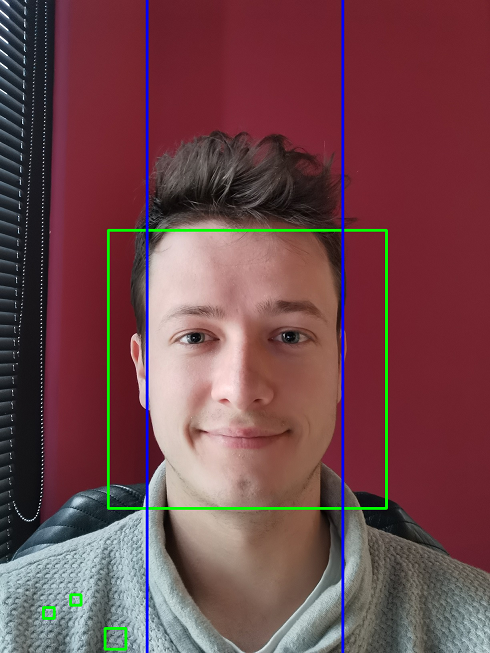
\includegraphics[scale=0.3]{img/face_section/face_filter_boundary_1.png}}
            \hspace{8mm}
            \subfigure[Po filtrowaniu]{\label{fig:face_boundary_after}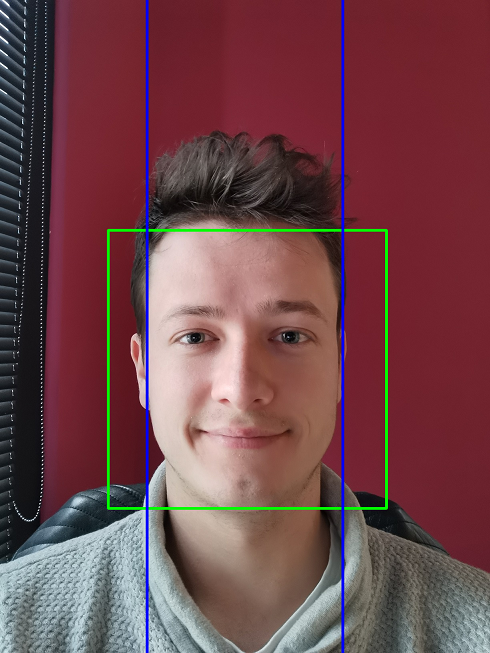
\includegraphics[scale=0.3]{img/face_section/face_filter_boundary_2.png}}
        \end{center}
        \caption{Działanie pierwszego etapu filtrowania detekcji twarzy w oparciu o jej położenie na zdjęciu.}
        \label{fig:face_boundary}
    \end{figure}
    
    \item Kolejnym etapem jest odrzucenie tych detekcji, które wychodzą zbyt daleko poza zdjęcie. Jeśli którykolwiek z~boków prostokąta wystaje pionowo/poziomo o~odległość większą niż $10\%$ odpowiednio wysokości/szerokości to zostaje odrzucony (\hyperref[{fig:face_out}]{rys.~\ref{fig:face_out}}).
    
    \begin{figure}[!h]
        \begin{center}
            \subfigure[Przed filtrowaniem zależnym od wystawania poza obraz]{\label{fig:face_out_before}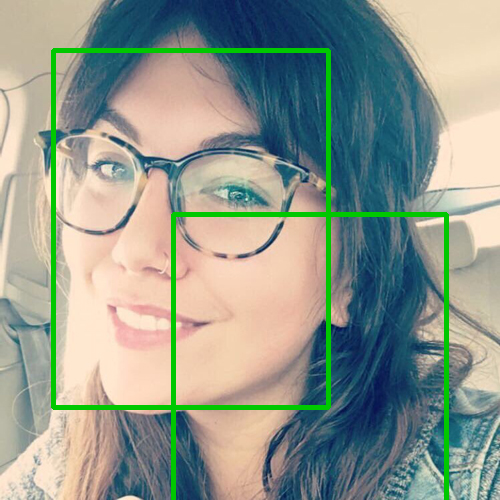
\includegraphics[scale=0.25]{img/face_section/face_filter_out_before.png}}
            \hspace{8mm}
            \subfigure[Po filtrowaniu]{\label{fig:face_out_after}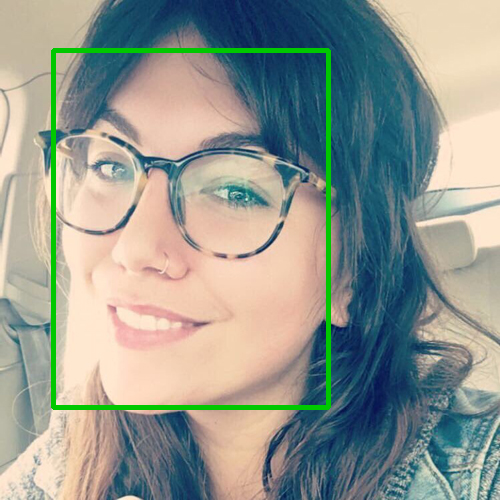
\includegraphics[scale=0.25]{img/face_section/face_filter_out_after.png}}
        \end{center}
        \caption{Działanie drugiego etapu filtrowania detekcji twarzy w oparciu o odległość wykrytego obszaru poza zdjęciem.}
        \label{fig:face_out}
    \end{figure}
    
    \item Z~pozostałych obszarów wybierany jest ten, który zajmuje największą powierzchnię. Taki wybór umotywowany jest własnymi obserwacjami autora na temat zachowania się algorytmów detekcji twarzy oraz tym, że~głowa użytkownika telefonu na obrazie z kamery przedniej zajmuje większą część płaszczyzny, ponieważ korzystając z~urządzenia nie trzymamy go bardzo daleko od siebie. (\hyperref[{fig:face_size}]{rys.~\ref{fig:face_size}})
    
    \begin{figure}[!h]
        \begin{center}
            \subfigure[Przed filtrowaniem zależnym od wielkości]{\label{fig:face_size_before}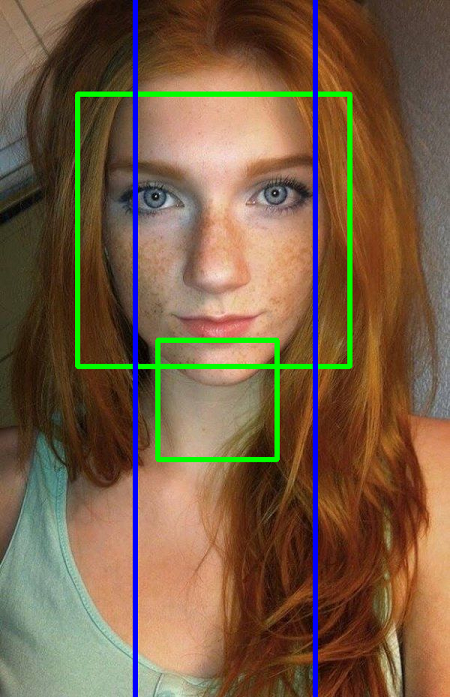
\includegraphics[scale=0.3]{img/face_section/face_filter_size_1.png}}
            \hspace{8mm}
            \subfigure[Po filtrowaniu]{\label{fig:face_size_after}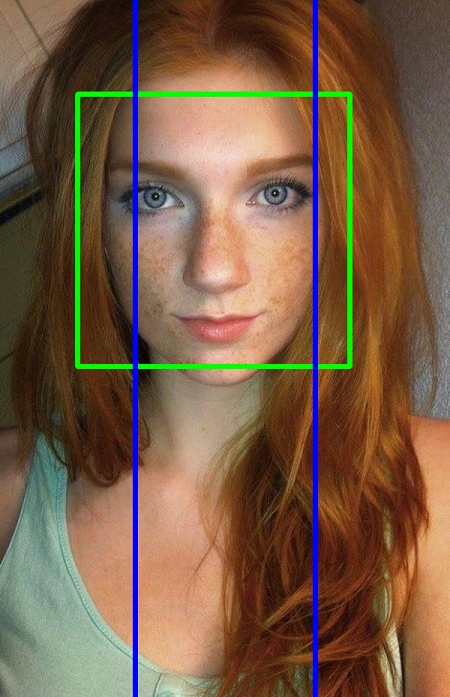
\includegraphics[scale=0.3]{img/face_section/face_filter_size_2.png}}
        \end{center}
        \caption{Działanie ostatniego etapu filtrowania detekcji twarzy w oparciu o wielkość wykrytego obszaru. Źródło zdj.: \cite{readheadPortrait1}}
        \label{fig:face_size}
    \end{figure}
    
    
    
\end{itemize}
\newpage

\section{Porównanie algorytmów detekcji twarzy}

W rozdziale \hyperref[{section:face_detection}]{\textit{\ref{section:face_detection}.Detekcja twarzy}} przedstawiłem kilka metod, które zostały zaimplementowane w projekcie. Ze względu, że dla prawidłowego i akceptowalnego działania aplikacji potrzebna jest odpowiednia skuteczność i szybkość detekcji twarzy, przetestuję i porównam wszystkie metody (z wyłączeniem \textit{CNN MMOD} - patrz rozdz. \hyperref[{section:no_cnn}]{\textit{\ref{section:no_cnn}}}). Na podstawie wyników wybiorę jedną, której będę używał w dalszej części projektu.


\subsection{Odrzucenie algorytmu Dlib CNN MMOD} \label{section:no_cnn}
Ze względu na bardzo wolne działanie algorytmu dlib opartego na konwolucyjnych sieciach neuronowych MMOD nie zostanie on przetestowany i zostaje od razu odrzucony. Czas przetwarzania jednego zdjęcia 500x500 wynosił kilka sekund, co całkowicie uniemożliwia działanie aplikacji w czasie rzeczywistym. Bardzo niska prędkość detekcji prawdopodobnie wynika z niemożności skorzystania z obliczeń na karcie graficznej na urządzeniach mobilnych. Metoda ta jest bardzo szybka gdy wykorzystuje do działania takie architektury jak CUDA \cite{nvidia_cuda}, natomiast dużo gorzej radzi sobie z obliczeniami wykonywanymi na procesorach CPU.

\subsection{Testowanie na statycznych zdjęciach}

Pierwszy etap testowania algorytmów detekcji twarzy będzie bazował na statycznych zdjęciach z głównego datasetu (patrz rozdz. \hyperref[section:dataset]{\textit{\ref{section:dataset}.Dataset}}). Pozwoli to przetestować na jednakowych danych wszystkie metody pod względem ich skuteczności wykrywania docelowych obszarów w różnych warunkach oraz uzyskać miarodajne wyniki.

\subsubsection{Oczekiwany wynik}

Każde zdjęcie z datasetu do tego etapu opisałem przez dwa prostokąty między którymi powinna się znaleźć wykryta przez algorytm twarz. Obszar ten został dobrany w następujący sposób:

\begin{itemize}
    \item Wewnętrzna część obejmuje minimalny obszar, na którym znajdują się brwi, oczy, nos i usta.
    \item W zewnętrznym prostokącie powinna znaleźć się cała twarz. Powiększony jest on o pewną tolerancję. 
\end{itemize}

\begin{figure}[!h]
    \begin{center}
        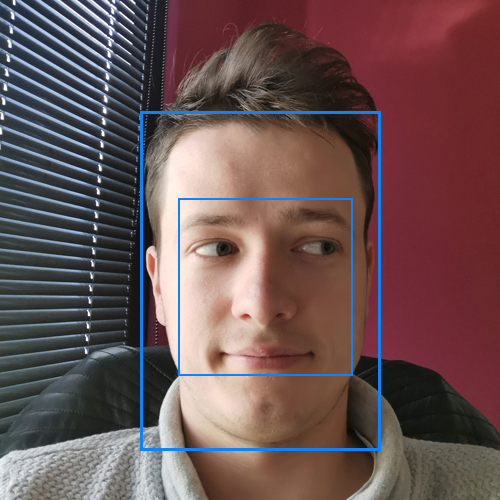
\includegraphics[scale=0.3]{img/face_section/face_test_expected.jpg}
        \caption{Oczekiwany obszar detekcji twarzy. }
        \label{fig:face_test_expected}
    \end{center}
\end{figure}

\subsubsection{Warunki testowania}

Dla każdego algorytmu zostaną przeprowadzone testy na zestawach obrazów o następujących rozdzielczościach i przestrzeniach barw:

\begin{itemize}
    \item 300x300 RGB
    \item 500x500 RGB
    \item 300x300 skala szarości
    \item 500x500 skala szarości
\end{itemize}

W przypadku \textit{DNN Caffe} nie jest możliwe przeprowadzenie badań dla zdjęć w skali szarości, ponieważ wymaga on obrazu z trzema kanałami barw.
\par
Testy będą przeprowadzone w trybie \textit{release}, ponieważ w trybie \textit{debuggowania} algorytm \textit{Dlib HOG} działał nawet $180$ razy wolniej. W przypadku pozostałych algorytmów tryb budowania nie miał większego wpływu na prędkość obliczeń, ale żeby wyniki były jak najbardziej miarodajne to każdy test musi być przeprowadzony w tych samych warunkach.







\subsubsection{Badanie skuteczności detekcji} \label{section:skutecznosc_detekcji_twarzy}

W tym teście zostaną zebrane i porównane następujące dane:
\begin{itemize}
    \item \textbf{Prawidłowe detekcje} - suma perfekcyjnych i częściowo dobrych detekcji
    \item \textbf{Perfekcyjne detekcje} - jeśli wykryty obszar w pełni znajduje się pomiędzy oczekiwanym prostokątami
    \item \textbf{Częściowo dobre detekcje} - jeśli są krawędzie, które znajdują się poza oczekiwanym obszarem, ale w zadowalającej odległości (patrz niżej - \hyperref[{uwaga:czesciowo_dobry}]{\textit{Uwaga 1.}})
    \item \textbf{Z 3 na 4 krawędzie perfekcyjne detekcje} - jeśli tylko jedna krawędź znajduje się poza oczekiwanym obszarem w zadowalającej odległości (patrz niżej - \hyperref[{uwaga:3_4_perfekcyjny}]{\textit{Uwaga 2.}})
    \item \textbf{Złe detekcje} - jeśli twarz nie została wykryta lub wskazany obszar jest niezadowalający
    \item \textbf{Twarze niewykryte} - jeśli całkowicie nie udało się wykryć twarzy (patrz niżej - \hyperref[{uwaga:dodatkowy_zle}]{\textit{Uwaga 3.}})
\end{itemize}

\textit{Uwaga 1.}\label{uwaga:czesciowo_dobry} Obszar uznany jest za częściowo dobry jeśli żadna krawędź nie jest oddalona o więcej niż $1.2x$ i maksymalnie jedna oddalona jest o długość z przedziału $[1.1x, 1.2x]$. Odległość $x$ to szerokość lub wysokość (zależnie od krawędzie) maksymalnego oczekiwanego obszaru twarzy.
\par
\textit{Uwaga 2.}\label{uwaga:3_4_perfekcyjny} Obszar zaliczony jest do grupy 3/4 perfekcyjnych detekcji, jeśli 3 krawędzie znajdują się w oczekiwanym obszarze, a czwarta odchylona od normy w przedziale $[1.0x, 1.2x]$.
\par 
\textit{Uwaga 3.}\label{uwaga:dodatkowy_zle} Dodatkowy podział złej detekcji na niewykryte twarze wynika z faktu, że metody oparte o \textit{Cascasding Classifier} na wyjściu podają obszar kwadratowy i przy rozciągniętej lub pochylonej twarzy boczne obszary mogą być bardzo oddalone od oczekiwanej wartości, ale dalej wykryć twarz. 

\vspace{10mm}

\begin{table}[!h]
\label{tab:face_detect_accuracy_RGB}
\centering
\caption{Skuteczność algorytmów detekcji twarzy dla obrazów RGB}
\resizebox{\textwidth}{!}{%
\begin{tabular}{|c|c|c|c|c|c|c|c|}
\hline
 &
  \textbf{\begin{tabular}[c]{@{}c@{}}Prawidłowe\\ detekcje\end{tabular}} &
  \textbf{\begin{tabular}[c]{@{}c@{}}Perfekcyjne\\ detekcje\end{tabular}} &
  \textbf{\begin{tabular}[c]{@{}c@{}}Częściowo\\ dobre\\ detekcje\end{tabular}} &
  \textbf{\begin{tabular}[c]{@{}c@{}}3/4\\ krawędzie\\ perfekcyjne\end{tabular}} &
  \textbf{\begin{tabular}[c]{@{}c@{}}Złe\\ detekcje\end{tabular}} &
  \textbf{\begin{tabular}[c]{@{}c@{}}Niewykryte\\ twarze\end{tabular}}  \\ \hline\hline
\textbf{Haar Cascade 500x500} &
  69 &
  4 &
  65 &
  32 &
  11 &
  9 \\ \hline
  
\textbf{Haar Cascade 300x300} &
 68 &
  5 &
  63 &
  33 &
  12 &
   9  \\ \hline
  
  \textbf{LBP Cascade 500x500} &
  58 &
  4 &
  54 &
  29 &
  22 &
  22 \\ \hline
  
  \textbf{LBP Cascade 300x300} &
  61 &
  4 &
  57 &
  34 &
  19 &
  17  \\ \hline
  
\textbf{DNN Caffe 500x500} &
  80 &
  68 &
  12 &
  11 &
  0 &
  0  \\ \hline
  
\textbf{DNN Caffe 300x300} &
  80 &
  62 &
  18 &
  18 &
  0 &
  0  \\  \hline
  
\textbf{Dlib HOG 500x500} &
  78 &
  31 &
  47 &
  36 &
  2 &
  2  \\  \hline
  
\textbf{Dlib HOG 300x300} &
  76 &
  24 &
  52 &
  33 &
  4 &
  4  \\  \hline
  
  \hline
\end{tabular}%
}
\end{table}
\begin{table}[!h]
\label{tab:face_detect_accuracy_GRAY}
\centering
\caption{Skuteczność algorytmów detekcji twarzy dla obrazów w skali szarości ze zbioru danych}
\resizebox{\textwidth}{!}{%
\begin{tabular}{|c|c|c|c|c|c|c|}
\hline
 &
  \textbf{\begin{tabular}[c]{@{}c@{}}Prawidłowe\\ detekcje\end{tabular}} &
  \textbf{\begin{tabular}[c]{@{}c@{}}Perfekcyjne\\ detekcje\end{tabular}} &
  \textbf{\begin{tabular}[c]{@{}c@{}}Częściowo\\ dobre\\ detekcje\end{tabular}} &
  \textbf{\begin{tabular}[c]{@{}c@{}}3/4\\ krawędzie\\ perfekcyjne\end{tabular}} &
  \textbf{\begin{tabular}[c]{@{}c@{}}Złe\\ detekcje\end{tabular}} &
  \textbf{\begin{tabular}[c]{@{}c@{}}Niewykryte\\ twarze\end{tabular}}   \\ \hline \hline
\textbf{Haar Cascade 500x500} &
  69 &
  4 &
  65 &
  31 &
  11 &
  9  \\ \hline

\textbf{Haar Cascade 300x300} &
  67 &
  4 &
  63 &
  34 &
  13 &
  9  \\ \hline
  
\textbf{LBP Cascade 500x500} &
  60 &
  5 &
  55 &
  30 &
  20 &
  17  \\ \hline
  
\textbf{LBP Cascade 300x300} &
  60 &
  4 &
  56 &
  31 &
  20 &
  17  \\ \hline
  
\textbf{DNN Caffe 500x500} &
  nd. &
  nd. &
  nd. &
  nd. &
  nd. &
  nd. \\ \hline
  
\textbf{DNN Caffe 300x300} &
  nd. &
  nd. &
  nd. &
  nd. &
  nd. &
  nd.  \\ \hline
  
  \textbf{Dlib HOG 500x500} &
  75 &
  27 &
  48 &
  35 &
  5 &
  5  \\ \hline
  
\textbf{Dlib HOG 300x300} &
  72 &
  23 &
  49 &
  31 &
  7 &
  7  \\ \hline
  
  \hline
\end{tabular}%
}
\end{table}

Metoda \textit{Haar Cascade} daje średnio $\sim69/80$ $(86\%)$ dobrych detekcji. Jest to dosyć przeciętny wynik. Na taki rezultat składa się kilka problemów tej metody. Nie radzi sobie ona dobrze z częściowo zakrytymi twarzami lub gdy głowa jest pochylona w bok. Kolejnymi czynnikiem wpływającym negatywnie na detekcje jest światło - problem z wykrywaniem występuje gdy zdjęcie jest zbyt jasne, twarz oświetlona lub źródło światła świeci prosto w obiektyw. Zaletą tej metody można zapisać małą ilość zwróconych przez nią dodatkowych, błędnych obszarów, które musiały zostać odfiltrowane.

\par
\textit{Klasyfikator kaskadowy} bazując na modelu \textit{LBP} miał najgorsze wyniki detekcji twarzy, na poziomie $\sim60/80$ $(75 \%)$. Jednak co zwraca uwagę to fakt, że bardzo duży odsetek twarzy nie został w ogóle wykryty. Występują tu te same problemy co w \textit{Haar Cascade}, ale dodatkowo algorytm nie radzi sobie gdy twarz zajmuje prawie całe zdjęcie.

\par
Najlepszy wynik detekcji uzyskał bezdyskusyjnie \textit{DNN Caffe}. Fakt, że w każdym z dwóch testów wykrył on $100 \%$ twarzy jest warty odnotowania. Co więcej perfekcyjne detekcje były na poziomie $\sim65/80$ $(81,25 \%)$. Nie występują tu problemy takie jak w poprzednich algorytmach. Radzi sobie on dobrze w złych warunkach oświetleniowych. Częściowe zakrycie twarzy nie wpływa na detekcję. Wykrywa on dobrze zarówno pochylone jak i odwrócone twarze. Jedynym negatywnym zjawiskiem, które zaobserwowałem w tej metodzie to zwracanie wielu dodatkowych obszarów, które są błędne. Zastosowanie filtrowania pozwoliło jednak odrzucić wszystkie błędne obszary.

\par
Bardzo dobre wyniki detekcji uzyskał również algorytm \textit{Dlib HOG}, w szczególności w przypadku zdjęć RGB 500x500 - jego skuteczność była na poziomie $78/80$ $(97,5 \%$). Zaletą tej metody jest zwracanie tylko jednego wykrytego obszaru - na żadnym z 80 zdjęć nie zwrócił ani jednego dodatkowego miejsca, które uznał za twarz. Nie udało się mu się wykryć twarzy gdy była ona w połowie zakryta. Zakładając jednak, że aplikacja będzie wykorzystywać oczy, usta itd. użytkownika przed telefonem można przyjąć, że jego twarz będzie w wystarczającym stopniu widoczna. W przeciwieństwie do pozostałych metod, które zwracają obszar całej twarzy, ta wykrywa częściowo obcięty rejon - np. pomijając czoło. Nie jest to w ogólności wadą, ponieważ te części twarzy nie są konieczne w pozostałych etapach.

\vspace{5mm}
Różnica w procencie perfekcyjnych detekcji pomiędzy \textit{DNN Caffe}, a pozostałymi wynika z rodzaju obszarów zwracanych przez te algorytmy. Metoda oparta na głębokich sieciach neuronowych zwraca prostokąt o dowolnym stosunku boków, natomiast reszta zwraca kwadrat. Dzięki temu \textit{DNN} lepiej dopasowuję się do kształtu twarzy niż \textit{Cascading Classifier} i \textit{HOG}.

\vspace{5mm}
Zmiana różnicy barw nie przyniosła istotnych zmian w skuteczności działania poszczególnych algorytmów. Jedynie zauważalne obniżenie detekcji w skali szarości w porównaniu do RGB widoczne jest dla metody opartej na \textit{histogramie gradientów zorientowanych Dlib}.

\subsubsection{Badanie szybkości detekcji}

W tym teście zostaną zebrane i porównane następujące dane:

\begin{itemize}
    \item \textbf{Całkowity czas przetwarzania} - suma czasów wszystkich 20 iteracji, całkowity czas testu.
    \item \textbf{Średni czas przetwarzania pojedynczej iteracji} - uśredniony czas pojedynczej iteracji
    \item \textbf{Średni czas przetwarzania jednego zdjęcia} - uśredniony czas przetwarzania pojedynczego zdjęcia
\end{itemize}

\par
\textit{Uwaga 1.}\label{uwaga:ilosc_powtorzen} Celem miarodajnego wyniku czasu przetwarzania każdy test zostanie przeprowadzony 20 razy.

\vspace{10mm}

\begin{table}[!h]
\label{tab:face_detect_speed_RGB}
\centering
\caption{Czas przetwarzania algorytmów detekcji twarzy dla obrazów RGB}

\begin{tabular}{|c|c|c|c|}
\hline
 & 
  \textbf{\begin{tabular}[c]{@{}c@{}}Całkowity czas \\ przetwarzania \end{tabular}} &
  \textbf{\begin{tabular}[c]{@{}c@{}}Średni czas\\ przetwarzania \\ pojedynczej iteracji\end{tabular}} &
  \textbf{\begin{tabular}[c]{@{}c@{}}Średni czas\\przetwarzania \\ pojedynczego\\zdjęcia\end{tabular}} \\ \hline\hline
\textbf{Haar Cascade 500x500} & 
  116,72 s &
  5,836 s &
  0,072 s    \\ \hline
  
\textbf{Haar Cascade 300x300} & 
  46,24 s &
  2,312 s &
  0,028 s     \\ \hline
  
  \textbf{LBP Cascade 500x500} & 
  63,27 s &
  3,163 s&
  0,039 s  \\ \hline
  
  \textbf{LBP Cascade 300x300} & 
  21,25 s &
  1,062 s &
  0,013 s    \\ \hline
  
\textbf{DNN Caffe 500x500} &
  106,17 &
  5,308 &
  0,066 s  \\ \hline
  
\textbf{DNN Caffe 300x300} & 
 103,56 s &
 5,178 s &
 0,064 s   \\  \hline
  
\textbf{Dlib HOG 500x500} & 
  71,10 s &
  3,555 s &
  0,044 s     \\  \hline
  
\textbf{Dlib HOG 300x300} & 
  26,08 s &
  1,304 s &
  0,016 s   \\  \hline
  
  \hline
\end{tabular}%

\end{table}
\begin{table}[!h]
\label{tab:face_detect_speed_GRAY}
\centering
\caption{Czas przetwarzania algorytmów detekcji twarzy dla obrazów w skali szarości ze zbioru danych.}

\begin{tabular}{|c|c|c|c|}
\hline
 & 
  \textbf{\begin{tabular}[c]{@{}c@{}}Całkowity czas \\ przetwarzania \end{tabular}} &
  \textbf{\begin{tabular}[c]{@{}c@{}}Średni czas\\ przetwarzania \\ pojedynczej iteracji\end{tabular}} &
  \textbf{\begin{tabular}[c]{@{}c@{}}Średni czas\\przetwarzania \\ pojedynczego\\zdjęcia\end{tabular}} \\ \hline\hline
\textbf{Haar Cascade 500x500} & 
  116,52 s &
  5,826 s &
  0,072 s    \\ \hline
  
\textbf{Haar Cascade 300x300} & 
  45,93 s &
  2,296 s &
  0,028 s     \\ \hline
  
  \textbf{LBP Cascade 500x500} & 
  62,34 s &
  3,117 s &
  0,038 s  \\ \hline
  
  \textbf{LBP Cascade 300x300} & 
  21,64 s &
  1,082 s &
  0,013 s    \\ \hline
  
\textbf{DNN Caffe 500x500} & 
  nd. &
  nd. &
  nd.  \\ \hline
  
\textbf{DNN Caffe 300x300} & 
  nd. &
  nd. &
  nd.   \\  \hline
  
\textbf{HOG 500x500} & 
  58,60 s &
  2,930 s &
  0,036 s     \\  \hline
  
\textbf{HOG 300x300} & 
  21,88 s &
  1,094 s &
  0,013 s   \\  \hline
  
  \hline
\end{tabular}%

\end{table}

Najszbyszy okazał się algorytm operujący na histogramach gradientowych. Niewiele wolniej przetwarzał algorytm kaskadowy \textit{LBP}. \textit{DNN Caffe} dla zdjęć $500x500$  był porównywalnie szybki jak \textit{Haar Cascade}, natomiast już w przypadku $300x300$ około $2.5$ razy wolniejszy.
\par
Co ciekawe i warte odnotowania to fakt, że algorytm \textit{DNN} przetwarzał prawie tak samo szybko obie rozdzielczości zdjęć. Można wysnuć tezę, że dla tej metody wielkość obrazu nie ma wpływu na szybkość przetwarzania. Ze względu, że taka właściwość może okazać się przydatna w perspektywie dalszych etapów projektu, zamierzam zbadać tę zależność w następnym rozdziale.
\par
Na szybkość detekcji algorytmu \textit{HOG} niewątpliwie miało wpływ użycie go w języku C++ mimo narzutu związanego z wywoływaniem go przez interfejs \textit{Java Native Interface}.

\vspace{5mm}

Zmiana detekcji z trójkanałowej RGB na skalę szarości w przypadku \textit{Haar} i \textit{LBP} nie skróciła czasu detekcji. W przypadku metody z biblioteki \textit{Dlib} algorytm przetwarzał te zdjęcia $\sim15-20 \%$ krócej niż w wersji kolorowej.


\subsubsection{Wpływ wielkości zdjęcia na szybkość algorytm \textit{DNN Caffe}}

\begin{table}[!h]
\label{tab:face_dnn_speed}
\centering
\caption{Wpływ rozdzielczości zdjęcia na detekcję DNN}
\resizebox{\textwidth}{!}{%
\begin{tabular}{|c|c|c|c|c|c|}
\hline
 &
  \textbf{\begin{tabular}[c]{@{}c@{}}Prawidłowe\\ detekcje\end{tabular}} &
  \textbf{\begin{tabular}[c]{@{}c@{}}Perfekcyjne\\ detekcje\end{tabular}} &
  \textbf{\begin{tabular}[c]{@{}c@{}}Częściowo\\ dobre\\ detekcje\end{tabular}} &
  \textbf{\begin{tabular}[c]{@{}c@{}}Średni czas\\ przetwarzania \\ pojedynczej iteracji\end{tabular}} &
  \textbf{\begin{tabular}[c]{@{}c@{}}Średni czas \\ przetwarzania\\ pojedynczego\\ zdjęcia\end{tabular}} \\ \hline
\textbf{300x300} &
  80 &
  62 &
  18 &
  5,148 s &
  0,064 s \\ \hline
  
\textbf{500x500} &
  80 &
  68 &
  12 &
  5,239 s &
  0,065 s \\ \hline
  
\textbf{1000x1000} &
  80 &
  67 &
  13 &
  5,29 s &
  0,066 s \\ \hline
  
  \textbf{2000x2000} &
  80 &
  65 &
  15 &
  4,988 s &
  0,062 s \\ \hline
 
  \hline
\end{tabular}%
}
\end{table}

Test ten potwierdza postawioną przeze mnie wcześniej tezę, że wielkość zdjęcia nie ma wpływu na szybkość przetwarzania algorytmu \textit{DNN Caffe}. Testy w każdej rozdzielczości zostały wykonane mniej więcej w tym samym czasie, a różnica zapewne jest skutkiem obciążenia urządzenia w danej chwili i jest pomijalna.\\
Prawdopodobnie wynika to z faktu, że metoda ta tworzy na podstawie zdjęcia wejściowego plamki o podanej wielkości niezależnie od rozdzielczości. W zaimplementowanym algorytmie jest to rozmiar 300x300. Dzięki temu zawsze ma on do przetworzenia taką samą ilość danych, więc czas powinien być w przybliżeniu stały. \\
Skuteczność detekcji w każdym wariancie była przybliżona i uzyskiwała $100 \%$ prawidłowych wskazań.

\subsubsection{Precyzja detekcji algorytmu \textit{DNN Caffe} zależnie od sposobu filtracji}

Metoda oparta na głębokich sieciach neuronowych na wyjściu zwraca wiele obszarów wraz ze wskaźnikiem pewności detekcji. Im większy współczynnik tym w teorii większa szansa, że jest to obiekt, który chcieliśmy wykryć.
\par
Z tego powodu postanowiłem porównać autorskie filtrowanie opisane wcześniej (patrz rozdz. \hyperref[{section:face_detection_filter}]{\textit{\ref{section:face_detection_filter}.Filtrowanie wyników}}) i wybór detekcji z największym procentem pewności.
\par

\vspace{8mm}

\begin{table}[!h]
\label{tab:face_filter_test}
\centering
\caption{Wynik porównania sposobów filtrowania detekcji twarzy algorytmem DNN Caffe na zbiorze danych.}
\resizebox{\textwidth}{!}{%
\begin{tabular}{|c|c|c|c|c|c|c|}
\hline
 &
  \textbf{\begin{tabular}[c]{@{}c@{}}Prawidłowe\\ detekcje\end{tabular}} &
  \textbf{\begin{tabular}[c]{@{}c@{}}Perfekcyjne\\ detekcje\end{tabular}} &
  \textbf{\begin{tabular}[c]{@{}c@{}}Częściowo\\ dobre\\ detekcje\end{tabular}} &
  \textbf{\begin{tabular}[c]{@{}c@{}}3/4\\ krawędzie\\ perfekcyjnie\end{tabular}} &
  \textbf{\begin{tabular}[c]{@{}c@{}}Złe\\ detekcje\end{tabular}} &
  \textbf{\begin{tabular}[c]{@{}c@{}}Niewykryte\\ twarze\end{tabular}}  \\ \hline \hline
\textbf{Autorskie filtrowanie 300x300} &
  80 &
  62 &
  18 &
  18 &
  0 &
  0  \\ \hline
  
\textbf{Autorskie filtrowanie  500x500} &
  80 &
  68 &
  12 &
  11 &
  0 &
  0  \\ \hline
  
\textbf{Najwyższy współczynnik pewności 300x300} &
  76 &
  58 &
  18 &
  18 &
  4 &
  4  \\ \hline

  \textbf{Najwyższy współczynnik pewności 500x500} &
  76 &
  64 &
  12 &
  11 &
  4 &
  4  \\ \hline
 
  \hline
\end{tabular}%
}
\end{table}

Wyniki w \hyperref[{tab:face_filter_test}]{\textit{tabeli 3.6}} pokazują, że zaproponowana przeze mnie wcześniej sekwencja filtrowania wykrytych obszarów daje lepsze rezultaty niż wybór najwyższego współczynnika pewności.


\subsection{Testowanie na obrazie z kamery na żywo} \label{section:face_detection_test_live}

W teście opartym na statycznych zdjęciach najlepsze okazały się algorytmy \textit{DNN} i \textit{HOG}, a dodatkowo ten drugi był również najszybszy. Z tego względu w próbie wykorzystującej obraz na żywo badane będą wyłącznie te dwa algorytmy, a pozostałe odrzucone.
\par
Obraz przechwytywany będzie w domyślnej rozdzielczości dla modułu CameraX - $640x480$. \cite{camerax}
\par
Oba algorytmy zostaną przetestowane w czterech różnych warunkach:
\begin{itemize}
    \item \textit{1.} w zwykłych, domowych warunkach oświetleniowych
    \item \textit{2.} w ciemnym miejscu
    \item \textit{3.} z intensywnym oświetleniem zza osoby 
    \item \textit{4.} z intensywnym oświetleniem zza urządzenia
\end{itemize}

Zostaną zebrane informacje o procencie klatek z wykrytą twarzą oraz chwilową i średnią ilość klatek na sekundę. 
\par
Każdy test będzie trwał 210 klatek, ale pierwsze i ostatnie 5 nie będzie branych pod uwagę przy wynikach. Związane są one z inicjalizacją algorytmów oraz ręcznego wyłączenia aplikacji przez co nie przenoszą w pełni wartościowych informacji.

\subsubsection{Skuteczność detekcji}

Sprawdzenie skuteczności algorytmów polega na zebraniu informacji na ilu klatkach z obrazu na żywo udało się wykryć twarz.

\begin{table}[!h]
\label{tab:face_detect_accuracy_live}
\centering
\caption{Skuteczność algorytmów detekcji twarzy dla obrazu na żywo z kamery.}
\begin{tabular}{|c|c|c|c|c|}
\hline
 \textbf{\begin{tabular}[c]{@{}c@{}}Warunki\end{tabular}} &
  \begin{tabular}[c]{@{}c@{}}1.\end{tabular} &
  \begin{tabular}[c]{@{}c@{}}2.\end{tabular} &
  \begin{tabular}[c]{@{}c@{}}3.\end{tabular} &
  \begin{tabular}[c]{@{}c@{}}4.\end{tabular}    \\ \hline \hline
\textbf{DNN Caffe RGB} &
  200 &
  200 &
  200 &
  200 \\ \hline

\textbf{HOG RGB} &
  200 &
  200 &
  200 &
  200 \\ \hline
  
\textbf{HOG sk. szaro.} &
  200 &
  200 &
  200  &
  200 \\ \hline

  \hline
\end{tabular}%

\end{table}

Jak widać oba algorytmy wykrywały w każdej odebranej klatce twarz. Potwierdzają to zarówno logi jak i podgląd na żywo podczas testu. 

\subsubsection{Szybkość detekcji}

Szybkość detekcji będzie porównana za pomocą średniej ilości klatek na sekundę. Jako, że w statystykach nie jest uwzględniany tylko czas detekcji, a działanie całej aplikacji to występują tu pewne narzuty czasowe związany z wyświetlaniem obrazu i rysowaniem na nich wykrytego obszaru celem podglądu testowanych parametrów na żywo. Jednak opóźnienie to występuje w każdym algorytmie i można uznać je za takie same.

\begin{table}[!h]
\label{tab:face_detect_speed_live}
\centering
\caption{Szybkość algorytmów detekcji twarzy dla obrazu na żywo z kamery [klatki/s]}
\begin{tabular}{|c|c|c|c|c|c|}
\hline
 \textbf{\begin{tabular}[c]{@{}c@{}}Warunki\end{tabular}} &
  \begin{tabular}[c]{@{}c@{}}1.\end{tabular} &
  \begin{tabular}[c]{@{}c@{}}2.\end{tabular} &
  \begin{tabular}[c]{@{}c@{}}3.\end{tabular} &
  \begin{tabular}[c]{@{}c@{}}4.\end{tabular} &
  \textbf{\begin{tabular}[c]{@{}c@{}}Średnia:\end{tabular}}\\ \hline \hline
\textbf{DNN rgb} &
  14,004 &
  14,298 &
  14,175 &
  14,270 &
  14,186  \\ \hline

\textbf{HOG rgb} &
  16,488 &
  16,224 &
  16,337 &
  16,400 &
  16,362 \\ \hline
  
\textbf{HOG sk. szaro.} &
  19,405 &
  19,546 &
  19,367 &
  19,796 &
  19,528 \\ \hline

  \hline
\end{tabular}%

\end{table}

Podobnie jak w testach na statystycznych zdjęciach algorytm \textit{HOG} okazał się szybszy od \textit{DNN Caffe}. W przypadku histogramu gradientów w oparciu o zdjęcie w skali szarości była to prędkość większa aż o $37 \%$.


\subsection{Wybór algorytmu}

W dalszej części projektu zdecydowałem się na korzystanie z algorytmu \textit{dlib HOG} do detekcji twarzy. W testach skuteczności okazał się on prawie tak samo skuteczny jak \textit{DNN Caffe}, ale zdecydowanie od niego szybszy. 
\par
Dodatkowo wybór padł na dostarczanie do detektora obrazu w skali szarości ze względu na zysk w ilości klatek na sekundę - dla barw mono był szybszy o $19 \%$ od wersji trójkanałowej.
\newpage

\section{Facemark} \label{section:landmarks}

\textit{Facemarks} (lub \textit{Face landmarks}) to punkty nakładane na twarz wokół interesujących obszarów - takich jak oczy, nos czy usta. Pozwalają określić położenie, rozmiar czy kształt tych obiektów. Mogą być również użyte do predykcji czy mamy zamknięte/otwarte oczy (patrz rozdz. \hyperref[section:EARsection]{\textit{\ref{section:EARsection}.EAR}}) lub czy się uśmiechamy. 

\begin{figure}[!h]
    \begin{center}
        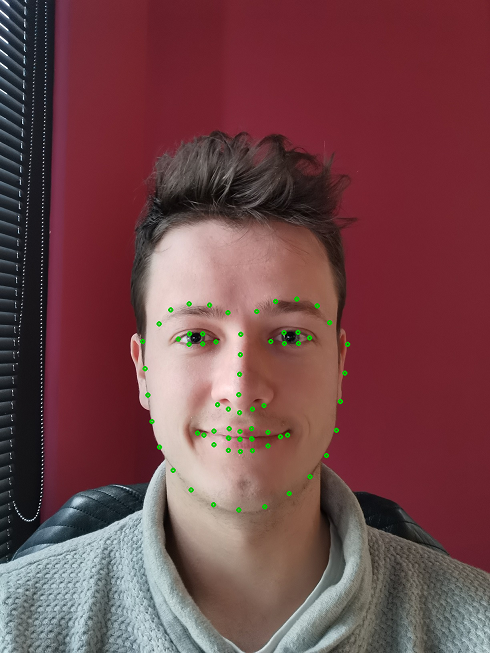
\includegraphics[scale=0.6]{img/landmark_section/landmarks_1.png}
        \caption{Przykład zdjęcia twarz z naniesionymi facemarkami}
        \label{fig:landmarks_1}
    \end{center}
\end{figure}

\subsection{Local binary features}
Metoda oparta o histogram LBF \cite{lbpFacemark}. W projekcie została użyta implementacja tego algorytmu z modułu \textit{face} \cite{opencvcontribface}, który zawarty jest w dodatkach do biblioteki OpenCV zbiorczo nazwanych \textit{contirb} \cite{opencv_contrib}. Do jej działania korzystałem z gotowego modelu \cite{lbpfacemarkmodel}, który był trenowany na datasecie \textit{HELEN} \cite{helen_dataset}.

\subsection{Kazemi}
Kolejnym algorytmem służącym do estymacji facemarków jest Kazemi \cite{kazemi}, który wykorzystuje drzewa regresyjne. Jest on zaimplementowany w bibliotece \textit{dlib}. Gotowy model był trenowany na podstawie datasetu \textit{iBUG 300-W face landmark} \cite{300Ibugdataset}.



\newpage

\section{Porównanie algorytmów detekcji znaczników twarzy}

Podobnie jak w~przypadku detekcji twarzy przeprowadzone zostały testy algorytmów wykrywania facemarków, przedstawionych w~rozdziale \hyperref[section:landmarks]{\ref{section:landmarks}}. Ze względu na specyfikę nanoszenia punktów charakterystycznych oraz ich ilość, trudno jest określić dokładność działania korzystając z~matematycznych i~liczbowych form wyrazu. Z~tego powodu ocena jakości obu algorytmów to subiektywna opinia autora na podstawie obserwacji znaczników obszaru oczu i~ust. Duża uwaga podczas opiniowania poświęcona została dokładności odwzorowaniu punktów w~przypadku przymkniętych lub całkiem zamkniętych oczu, ponieważ ma to istotny wpływ na inne aspekty pracy dyplomowej. Natomiast złożoność czasowa jest już mierzalna i~została wyrażona liczbowo. 




\subsection{Testowanie na statycznych zdjęciach}

Oba algorytmy zostały przetestowane na statycznych zdjęciach z~ze~zbioru danych w~zakresie skuteczności i~szybkości działania.

\subsubsection{Usunięcie części zdjęć ze zbioru danych}

Ze względu na wybór algorytmu \textit{HOG} do detekcji twarzy konieczne okazało się odrzucenie 2~z~80 przygotowanych zdjęć, ponieważ metodzie tej nie udało się wykryć na nich twarzy (patrz rozdz.~\hyperref[{section:skutecznosc_detekcji_twarzy}]{\textit{\ref{section:skutecznosc_detekcji_twarzy}}}).

\subsubsection{Badanie skuteczności detekcji}

Podczas testu zostały zebrane następujące dane:

\begin{itemize}
    \item \textbf{Prawidłowe detekcje} - pokrycie twarzy znacznikami, które uznane zostały za dobre
    \item \textbf{Złe detekcje} - pozostałe, które nie zostały uznane za dobre
    \item \textbf{Detekcje lepsze niż drugiego algorytmu} - który z~dwóch algorytmów poradził sobie lepiej w danym przypadku testowym. 
\end{itemize}

Zebrane dane są całkowicie subiektywnym odczuciem i~inne osoby mogą  mieć odmienną opinię oraz wyniki.

\vspace{5mm}

Oba algorytmy dawały taki sam rezultat zarówno w~skali szarości jak i~w~trzy kanałowym zestawie barw, dlatego tabela wynikowa została uproszczona przez usunięcie takiego podziału.

\begin{table}[!h]
\label{tab:facemarks_accuracy}
\centering
\caption{Skuteczność algorytmów detekcji landmarków}
\begin{tabular}{|c|c|c|c|}
\hline
 &
  \textbf{\begin{tabular}[c]{@{}c@{}}Prawidłowe\\ detekcje\end{tabular}} &
  \textbf{\begin{tabular}[c]{@{}c@{}}Złe\\ detekcje\end{tabular}} &
  \textbf{\begin{tabular}[c]{@{}c@{}}Detekcje lepsze niż\\ drugiego algorytmu\end{tabular}}   \\ \hline \hline
\textbf{LBF} &
  35 &
  42 &
  16 \\ \hline

\textbf{Kazemi} &
  66 &
  12 &
  62 \\ \hline
 
  
  \hline
\end{tabular}%
\end{table}

Zebrane dane pokazują jasno, że model oparty na metodzie \textit{Kazemi} dał zdecydowanie lepsze wyniki niż drugi badany algorytm. W~62 przypadkach testowych pokrycie twarzy facemarkami było subiektywnie dokładniejsze niż w~metodzie \textit{LBF}. Tylko~12~z~78 detekcji uznałem za błędne. Można przyjąć, że jest to wynik co najmniej poprawny.

\par

Kazemi dobrze radził sobie z~obróconymi i~pochylonymi twarzami, natomiast LBF w~takich przypadkach okazywał się mocno niedokładny i~nakładał znaczniki w sposób podobny jak dla twarzy ustawionych pionowo. Oba algorytmy miały problem w przypadku gdy cień padał na obszar oczu, wtedy znaczniki w~tych rejonach były odchylone od prawidłowych pozycji. Metoda LBF miała problem w~przypadku osób z~ciemniejszymi odcieniami skóry, a~także gdy proporcje twarzy były rozciągnięte. Gdy osoba na zdjęciu nosiła okulary nie wpływało to znacząco na dokładność algorytmu Kazemi w przeciwieństwie do drugiej metody, która osiągała wtedy złe rezultaty. Rozwiązanie LBF natomiast radziło sobie lepiej jeśli twarz i~oczy były częściowo zasłonięte. W~obu przypadkach trudne i~intensywne warunki oświetleniowe wpływały negatywnie na dokładność odwzorowania punktów charakterystycznych. 

\par

Metoda LBF myliła się na wielu zdjęciach bardzo mocno, a~punkty były rozłożone chaotycznie i~losowo. W tych przypadkach trudno oszacować powód, ale jest to fakt praktycznie dyskwalifikujący to rozwiązanie. Ma to odwzorowanie również w~tabeli, gdzie mniej niż połowa wyników została uznanych za dobre. 





\subsubsection{Badanie szybkości detekcji}

W~tym teście zostały zebrane i~porównane następujące dane:

\begin{itemize}
    \item \textbf{Całkowity czas przetwarzania} - suma czasów detekcji znaczników dla wszystkich 20 iteracji
    \item \textbf{Średni czas przetwarzania pojedynczej iteracji} - uśredniony czas detekcji znaczników dla pojedynczej iteracji
    \item \textbf{Średni czas przetwarzania jednego zdjęcia} - uśredniony czas detekcji znaczników dla pojedynczego zdjęcia
\end{itemize}

\begin{table}[!h]
\label{tab:facemarks_speed}
\centering
\caption{Czas przetwarzania algorytmów detekcji znaczników twarzy na zbiorze danych}

\begin{tabular}{|c|c|c|c|}
\hline
 & 
  \textbf{\begin{tabular}[c]{@{}c@{}}Całkowity czas \\ przetwarzania \end{tabular}} &
  \textbf{\begin{tabular}[c]{@{}c@{}}Średni czas\\ przetwarzania \\ pojedynczej iteracji\end{tabular}} &
  \textbf{\begin{tabular}[c]{@{}c@{}}Średni czas\\przetwarzania \\ pojedynczego\\zdjęcia\end{tabular}} \\ \hline\hline
  
\textbf{Kazemi RGB} & 
  5,717 s &
  0,285 s &
  0,00366 s    \\ \hline
  
\textbf{LBF RGB} & 
  6,545 s &
  0,327 s &
  0,00419 s  \\ \hline
  
\textbf{Kazemi sk. szaro.} & 
  5,472 s &
  0,273 s &
  0,00351 s     \\ \hline
  
\textbf{LBF sk. szaro.} & 
  6,084 s &
  0,304 s &
  0,00391 s    \\ \hline
  
  \hline
\end{tabular}%

\end{table}

Algorytm Kazemi z~użyciem biblioteki dlib i~języka C++ okazał się szybszy o~ponad $10\%$ od odpowiednika w postaci LBF. Obie metody uzyskały lepszy czas w~teście opartym na obrazach w~skali szarości niż w~RGB o~kilka procent. Istotnym faktem jest, że oba algorytmy potrzebują mało czasu (rząd wielkości $10^{-3} s$) na przetworzenie pojedynczego zdjęcia, dzięki czemu w~warunkach czasu rzeczywistego nie powodują znacznego spadku klatek na sekundę. 

\subsection{Testowanie na obrazie z kamery na żywo}

Kolejnym etapem testowania detekcji punktów charakterystycznych twarzy było wykorzystanie obrazu z~kamery na żywo. Warunki przeprowadzenia eksperymentu zostały określone w rozdz.~\hyperref[{section:face_detection_test_live}]{\ref{section:face_detection_test_live}}.

\subsubsection{Badanie skuteczność detekcji} \label{section:facemark_live_detection}

Ze względu na opisaną wyżej trudność matematycznego wyrażenia skuteczności nakładania znaczników, wyniki porównania zostały przedstawione w formie opisowej i~są subiektywnym odczuciem autora na podstawie obserwacji działania algorytmu na żywo.

\vspace{5mm}

Algorytm Kazemi bez zarzutu poradził sobie w~trzech scenariuszach. Natomiast w~jednym - przy mocnym oświetleniu padającym na obiektyw i~na twarz - występowało wtedy chwilowe niedokładne dopasowanie. Poza tym problemem radził sobie on bardzo dobrze. Ruchy twarzy nie przeszkadzały w prawidłowym ułożeniu znaczników. Punkty były bardzo stabilne, a~podczas sztywnego położenia twarzy nie występowały ich drgania.

\par

Gorsze wyniki uzyskała metoda LBF. Podobnie jak Kazemi miał pewne problemy podczas scenariusza opartego na mocnym oświetleniu. Występowało ciągłe drganie punktów, nawet podczas sztywnego położenia twarzy. Metoda ta oznaczała twarz jako szerszą niż w~rzeczywistości była. Podczas ruchów twarzy algorytm gubił prawidłowe położenie punktów.

\par

W obu przypadkach potwierdzają się problemy z~testów na statycznych zdjęciach, gdzie intensywne oświetlenie negatywnie wpływało na odwzorowanie punktów charakterystycznych. 

\subsubsection{Badanie szybkość detekcji} \label{section:facemark_speed_live}

Test był przeprowadzony używając detekcji twarzy \textit{HOG}, do którego dostarczano obraz w~przestrzeni barw RGB. 

\begin{table}[!h]
\label{tab:facemarks_speed_live}
\centering
\caption{Szybkość algorytmów detekcji znaczników twarzy dla obrazu na żywo z kamery [klatki/s]}
\begin{tabular}{|c|c|c|c|c|c|}
\hline
 \textbf{\begin{tabular}[c]{@{}c@{}}Warunki\end{tabular}} &
  \begin{tabular}[c]{@{}c@{}}1.\end{tabular} &
  \begin{tabular}[c]{@{}c@{}}2.\end{tabular} &
  \begin{tabular}[c]{@{}c@{}}3.\end{tabular} &
  \begin{tabular}[c]{@{}c@{}}4.\end{tabular} &
  \textbf{\begin{tabular}[c]{@{}c@{}}Średnia:\end{tabular}}\\ \hline \hline
\textbf{LBF RGB} &
  16,076 &
  15,960 &
  15,820 &
  16,079 &
  15,983  \\ \hline

\textbf{LBF sk. szaro.} &
  15,959 &
  16,016 &
  15,829 &
  15,793 &
  15,899 \\ \hline
  
\textbf{Kazemi RGB} &
  15,887 &
  15,941 &
  16,077 &
  16,171 &
  16,019  \\ \hline
  
\textbf{Kazemi sk. szaro.} &
  15,747 &
  16,146 &
  15,866 &
  16,096 &
  15,963 \\ \hline

  \hline
\end{tabular}%

\end{table}

Mniejsza ilość klatek w~przypadku testów w skali szarości prawdopodobnie jest związany z dodatkowym narzutem czasowym w~postaci konwersji obrazu z~trójkanałowej barwy na jednokanałową.

\par

Oba algorytmy uzyskały bardzo zbliżone wyniki. Niewiele szybsza okazała się jednak metoda Kazemi. Rezultat jest porównywalny z~testem przeprowadzonym na statycznych zdjęciach.





\subsection{Wybór algorytmu detekcji znaczników twarzy}

\textit{Kazemi} okazał się przede wszystkim dużo skuteczniejszym i~stabilnym algorytmem niż detekcja znaczników oparta na \textit{Local Binary Features}. Dodatkowo jest on około~$10\%$ szybszy. Wszystkie testy wskazują na wyższość \textit{Kazemi} i~z~tych powodów jest on używany w dalszej części pracy dyplomowej i~projektu, jako główny algorytm określenia położenia punktów charakterystycznych. 
\newpage

\section{EAR - Eye Aspect Ratio}
Metoda polegająca na obliczeniu \textit{EAR}  \cite{EARRaspberryPi} \cite{eyeBlinkEARRosebrock}, czyli stosunek otwarcia oczu - wysokość do szerokości widocznej części gałki ocznej. Wykorzystuje się tu landmarki (patrz rozdz. \hyperref[{section:landmarks}]{\textit{\ref{section:landmarks}.Landmarks}}) naniesione dookoła oczu.

\subsection{Wzór obliczania EAR}
Zależnie od ilości punktów wokół oka będzie różny wzór obliczania EAR.\\
Dla 6 punktów:
\begin{align}
    EAR = \frac{dist(L_0, L_1) + dist(L_2, L4)}{2 * dist(L_3, L_5)}
\end{align}
\\
Natomiast, dla 4 punktów:
\begin{align}
    EAR = \frac{dist(L_0, L_2)}{dist(L_1, L_3)}
\end{align}

Gdzie \textit{$L_x$} to kolejne landmarki dokoła oczu, a \textit{dist} to odległość między dwoma punktami (odległość euklidesowa).\\

\subsection{Zasada działania EAR w kontekście mrugania}

W teorii otwarte oczy będą miały większy wymiar liczbowy EAR, niż oczy zamknięte. Na \hyperref[{fig:theoretical_eye_landmarks}]{\textit{rysunku \ref{fig:theoretical_eye_landmarks}}} widać, że oko otwarte ma większe odległości między punktami pionowymi niż w przypadku  oka zamkniętego. Dzięki takim różnicą możemy wykryć spadek wskaźnika EAR poniżej pewnego ustalonego poziomu oznaczający zamknięcie oka, natomiast wzrost otwarcie oka. Całościowo obserwując zmiany np. za pomocą pochodnej jesteśmy w stanie stwierdzić mrugnięcie.

\begin{figure}[!h]
    \begin{center}
        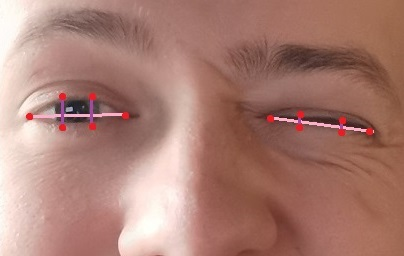
\includegraphics[scale=0.35]{img/landmark_section/theoretical_eye_landmarks.jpg}
        \caption{Teoretyczny rozmieszczene landmarków wokół oczu wraz z naniesionymi połączeniami do obliczenia EAR}
        \label{fig:theoretical_eye_landmarks}
    \end{center}
\end{figure}


\subsection{Testowanie z użyciem landmarków LBF opencv-contrib
}

\subsubsection{Test z użyciem kamery na żywo}

Wykonałem kilka krótkich testów z użyciem obrazu pochodzącego z przedniej kamery telefonu. 
\\
Poniżej znajdują się trzy testy, na których mrugnąłem tylko raz - lewym okiem, prawym i oboma na raz.

\begin{figure}[!h]
    \centering
    \begin{tikzpicture}
        \begin{axis}[
            xlabel = {Nr klatki obrazu z kamery},
            ylabel = {EAR},
            height = 0.5\linewidth,
            width = \linewidth,
            ymin= {0.10},
            ymax={0.30},
            ytick = {0.10, 0.12, 0.14, 0.16, 0.18, 0.20, 0.22, 0.24, 0.26, 0.28, 0.30},
            ymajorgrids = {true},
        ]
            \addplot[color=blue, mark=square*] table [x=x, y=a, col sep=comma] {csv/ear_left_1.csv};
            \addplot[color=red, mark=square*] table [x=x, y=b, col sep=comma] {csv/ear_left_1.csv};
        \end{axis}
    \end{tikzpicture}
    \caption{Mrugnięcie lewym okiem}
    \label{fig:left_eye_blink}
\end{figure}


\begin{figure}[!h]
    \centering
    \begin{tikzpicture}
        \begin{axis}[
            xlabel = {Nr klatki obrazu z kamery},
            ylabel = {EAR},
            height = 0.5\linewidth,
            width = \linewidth,
            ymin= {0.10},
            ymax={0.30},
            ytick = {0.10, 0.12, 0.14, 0.16, 0.18, 0.20, 0.22, 0.24, 0.26, 0.28, 0.30},
            ymajorgrids = {true},
        ]
            \addplot[color=blue, mark=square*] table [x=x, y=a, col sep=comma] {csv/ear_right_1.csv};
            \addplot[color=red, mark=square*] table [x=x, y=b, col sep=comma] {csv/ear_right_1.csv};
        \end{axis}
    \end{tikzpicture}
    \caption{Mrugnięcie prawym okiem}
    \label{fig:right_eye_blink}
\end{figure}

\begin{figure}[!h]
    \centering
    \begin{tikzpicture}
        \begin{axis}[
            xlabel = {Nr klatki obrazu z kamery},
            ylabel = {EAR},
            height = 0.5\linewidth,
            width = \linewidth,
            ymin= {0.10},
            ymax={0.30},
            ytick = {0.10, 0.12, 0.14, 0.16, 0.18, 0.20, 0.22, 0.24, 0.26, 0.28, 0.30},
            ymajorgrids = {true},
        ]
            \addplot[color=blue, mark=square*] table [x=x, y=a, col sep=comma] {csv/ear_both_1.csv};
            \addplot[color=red, mark=square*] table [x=x, y=b, col sep=comma] {csv/ear_both_1.csv};
        \end{axis}
    \end{tikzpicture}
    \caption{Mrugnięcie oboma oczami na raz}
    \label{fig:both_eyes_blink}
\end{figure}


Testy z pojedynczym mruganiem w krótkim okresie czasu dają przyzwoite wyniki i można na nich okreslić moment mrugania. W szczególności przy mrugnięciu jednym okiem.\\

Poniżej rozciągnąłem w czasie test na sekwencje kilku mrugnięć.

\begin{figure}[!h]
    \centering
    \begin{tikzpicture}
        \begin{axis}[
            xlabel = {Nr klatki obrazu z kamery},
            ylabel = {EAR},
            height = 0.5\linewidth,
            width = \linewidth,
            ymin= {0.10},
            ymax={0.30},
            ytick = {0.10, 0.12, 0.14, 0.16, 0.18, 0.20, 0.22, 0.24, 0.26, 0.28, 0.30},
            ymajorgrids = {true},
        ]
            \addplot[color=blue, mark=square*] table [x=x, y=a, col sep=comma] {csv/ear_long_1.csv};
            \addplot[color=red, mark=square*] table [x=x, y=b, col sep=comma] {csv/ear_long_1.csv};
        \end{axis}
    \end{tikzpicture}
    \caption{Kilka mrugnięć}
    \label{fig:multi_blinks_1}
\end{figure}

\begin{figure}[!h]
    \centering
    \begin{tikzpicture}
        \begin{axis}[
            xlabel = {Nr klatki obrazu z kamery},
            ylabel = {EAR},
            height = 0.5\linewidth,
            width = \linewidth,
            ymin= {0.10},
            ymax={0.30},
            ytick = {0.10, 0.12, 0.14, 0.16, 0.18, 0.20, 0.22, 0.24, 0.26, 0.28, 0.30},
            ymajorgrids = {true},
        ]
            \addplot[color=blue, mark=square*] table [x=x, y=a, col sep=comma] {csv/ear_long_2.csv};
            \addplot[color=red, mark=square*] table [x=x, y=b, col sep=comma] {csv/ear_long_2.csv};
        \end{axis}
    \end{tikzpicture}
    \caption{Kilka mrugnięć}
    \label{fig:multi_blinks_2}
\end{figure}

\begin{figure}[!h]
    \centering
    \begin{tikzpicture}
        \begin{axis}[
            xlabel = {Nr klatki obrazu z kamery},
            ylabel = {EAR},
            height = 0.5\linewidth,
            width = \linewidth,
            ymin= {0.10},
            ymax={0.30},
            ytick = {0.10, 0.12, 0.14, 0.16, 0.18, 0.20, 0.22, 0.24, 0.26, 0.28, 0.30},
            ymajorgrids = {true},
        ]
            \addplot[color=blue, mark=square*] table [x=x, y=a, col sep=comma] {csv/ear_long_3.csv};
            \addplot[color=red, mark=square*] table [x=x, y=b, col sep=comma] {csv/ear_long_3.csv};
        \end{axis}
    \end{tikzpicture}
    \caption{Kilka mrugnięć}
    \label{fig:multi_blinks_3}
\end{figure}

Tu również z dużym prawdopodobieństwem można okreśilć, w których klatkach wystąpiło mrugnięcie - widać gwałtowne obniżenie wartości EAR.
\\
Najlepsze wyniki były w przypadku pierwszego testu, ponieważ widać wtedy znaczną różnicę EAR między otwartym ($\sim0.26 - 0.30$), a zamkniętym okiem ($\sim0.12-0.18$). Na pozostałych testach różnice nie były już tak znaczące - na ostatnich dwóch wykresach otwarte i zamknięte oko ma niewielką różnicę w EAR. Takie małe różnice wyników mogą uniemożliwić prawidłową detekcję.

\vspace{3mm}
W każdym z przypadków testowych EAR dla jednego i drugiego oka prawie się pokrywają. Nawet przy mruganiu tylko jednym. Nie pozwoli to więc okręślić, którym okiem użytkownik mrugał.

\vspace{3mm}

Niewątpliwą trudnością w przypadku tej metody byłoby określenie progu wartości EAR, które zakwalifikowałbym jako mrugnięcie. Patrząc na wykresy powyżej można by przyjąć, że jest to wartość koło $~0.18$. Jednak w przypadku ostatecznego wyboru tej metody wymagałoby to dodatkowych badań celem określenia tej wartości.


\subsubsection{Niedokładność nakładania landmarków}

Patrząc jednak na położenie tych landmarków wokół oczu mam wątpliwości co do skuteczności tej metody:

\begin{figure}[!h]
    \begin{center}
        \subfigure[]{\label{fig:landmarks_accuracy_1}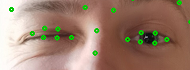
\includegraphics[scale=1.6]{img/landmark_section/landmarks_accuracy_1.png}}
        \hspace{8mm}
        \subfigure[]{\label{fig:landmarks_accuracy_2}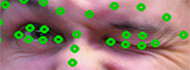
\includegraphics[scale=1.6]{img/landmark_section/landmarks_accuracy_2.png}}
    \end{center}
    \caption{Landmarki na oczach otwartych/zamkniętych}
    \label{fig:landmarks_accuracy_}
\end{figure}

Jak widać algorytm całkiem dobrze radzi sobie z rozmieszczeniem landmarków w przypadku otwartych oczu. Natomiast gdy oczy są zamknięte widać dużą niedokładność, która na pewno w dużym stopniu utrudnia prawidłową detekcję mrugnięcia.
\newpage

\section{Detekcja oczu} \label{section:eye_detection}

W tej pracy dyplomowej dużą role odgrywają oczy i ich wpływ na sterowanie aplikacją. Z tego powodu musiała zostać określona i zaimplementowana skuteczna metoda ich detekcji.



\subsection{Algorytmy detekcji oczu}

Na potrzeby tego etapu zostały zastosowane dwie metody opierające się na algorytmach opisanych wcześniej - klasyfikatory kaskadowe oraz facemarki.

\subsubsection{Klasyfikator kaskadowy Haar}

Metody detekcji oparte na klasyfikatorach kaskadowych zostały opisane w rozdz. \hyperref[{section:face_casacde_classifier}]{\textit{\ref{section:face_casacde_classifier}}}. Do detekcji oczu z użyciem tego algorytmu zostanie wykorzystany model autorstwa Shameem Hameed \cite{eye_haar_model}.

\subsubsection{Facemarki}

Opisane w rozdz. \hyperref[section:landmarks]{\ref{section:landmarks}} facemarki nanoszą punkty charakterystyczne na obraz twarzy. Znajdują się one m.in. wokół oczu. Fakt ten można wykorzystać do detekcji ich obszaru. Celem uzyskania takiego efektu należy wyznaczyć prostokąt, który będzie otaczał wszystkie sześć facemarków danego oka. \cite{detect_eye_facemarks}
\par
Przykład takiego działania widoczny jest na rysunku \ref{fig:facemarki_to_detect_eyes}.

\begin{figure}[!h]
    \begin{center}
        \subfigure[Facemarki wokół oka]{\label{fig:facemarki_to_detect_eyes_no_rect}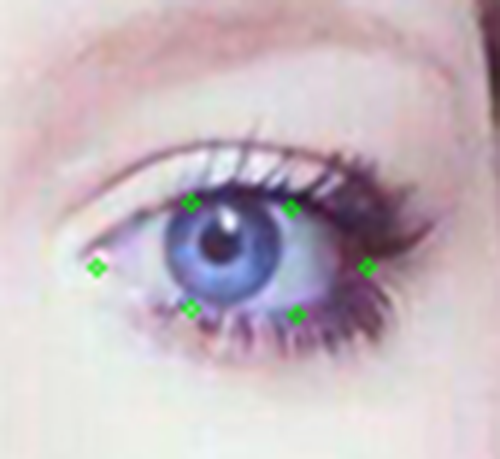
\includegraphics[scale=0.25]{img/eye_section/eye_facemarks.png}}
        \hspace{8mm}
        \subfigure[Naniesiony prostokąt otaczający facemarki wokół oka]{\label{fig:facemarki_to_detect_eyes_rect}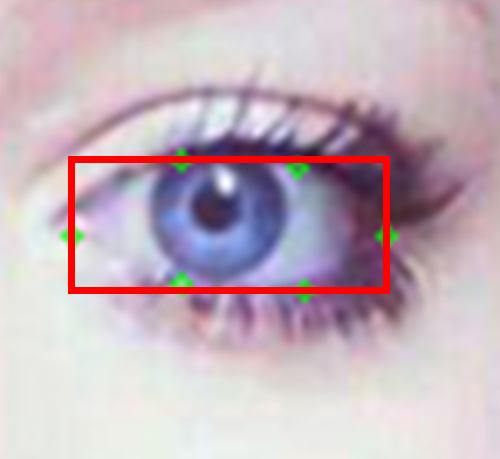
\includegraphics[scale=0.25]{img/eye_section/eye_facemarks_rect.png}}
    \end{center}
    \caption{Wykorzystanie facemarków do detekcji obszaru oczu}
    \label{fig:facemarki_to_detect_eyes}
\end{figure}

Wykorzystywany jest tu też wskaźnik \textit{EAR} (patrz rozdz. \hyperref[{section:EARsection}]{\textit{\ref{section:EARsection}. EAR - Eye Aspect Ratio}}) do wykrycia czy oko jest zamknięte czy otwarte.
\par
Skuteczność tej metody zależy od dokładności algorytmu odwzorowującego facemarki. Ewentualne niedoskonałości można niwelować zwiększając wielkość prostokąta o pewną tolerancję. Taki współczynnik w projekcie został testowo ustalony, a wyniki i wartości parametrów opisane w rozdz. \hyperref[{section:facemark_eye_size}]{\textit{\ref{section:facemark_eye_size}}}.



\subsection{Filtrowanie wyników metody Haar}

Ze względu, że algorytmu Haar może zwracać większą ilość prawdopodobnych obszarów, w których spodziewa się on wykryć pożądany obiekt, wprowadziłem filtrowanie wyników detekcji oczu. \\
Algorytm filtrowania składa się z dwóch etapów:

\begin{itemize}
    \item Podzielenie wykrytych obszarów na dwie grupy - na lewą i prawą stronę twarzy
    \item W obu grupach wybranie największego obszaru
\end{itemize}


Dodatkowo pozwoliło to na łatwe zidentyfikowanie który obszar to które oko i ich posortowanie.
\par
Przykładowy rezultat takiego filtrowania pokazany jest na \hyperref[{fig:eye_filter}]{\textit{rysunku \ref{fig:eye_filter}}}. 


\begin{figure}[!h]
    \begin{center}
        \subfigure[Przed filtrowaniem]{\label{fig:eye_filter_before}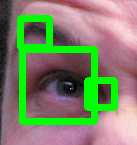
\includegraphics[scale=1.0]{img/eye_section/eye_filter_before.png}}
        \hspace{8mm}
        \subfigure[Po filtrowaniu]{\label{fig:eye_filter_after}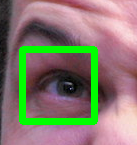
\includegraphics[scale=1.0]{img/eye_section/eye_filter_after.png}}
    \end{center}
    \caption{Efekt filtrowania obszarów detekcji oczu}
    \label{fig:eye_filter}
\end{figure}

\subsection{Obcięcie obszaru detekcji dla metody Haar}

Dla metody opartej na Haar zdecydowałem się dodatkowo zawęzić płaszczyznę przeszukiwań na niecałą twarz, celem uzyskania wyników lepszych niż bez takiego zmniejszenia. 
\par
Ustalenie jaki obszar da najlepszy rezultat odbyło się przez testowe sprawdzanie kombinacji trzech parametrów oznaczających jaka część wykrytej twarzy zostaje obcięta z poszczególnej strony. Mogą one przyjmować wartości w następujących przedziałach:

\begin{itemize}
    \item Góra: $[0.0,$ $0.02]$
    \item Dół: $[0.2,$ $0.6]$
    \item Boki: $[0.0,$ $0.02]$
\end{itemize}

Każdy parametr mógł osiągać wartości będące wielokrotnością $0.05$ w poszczególnych przedziałach.

\par

Ze względu na dużą ilość kombinacji ($225$) nie zostaną podane wyniki, a jedynie wybrana najlepsza kombinacja:
\begin{itemize}
    \item Góra: $0.05$
    \item Dół: $0.3$
    \item Boki: $0.0$
\end{itemize}

Algorytm Haar uzyskał lepszą skuteczność detekcji wykorzystując dodatkowe obcięcie niż bez niego:

\begin{table}[!h]

\centering
\caption{Skuteczność algorytmu detekcji oczu Haar z dodatkowym obcięciem i bez}
\label{tab:eye_haar_crop_result}
\resizebox{\textwidth}{!}{%
\begin{tabular}{|c|c|c|c|c|c|c|}
\hline
 &
  \textbf{\begin{tabular}[c]{@{}c@{}}Prawidłowe\\ detekcje\end{tabular}} &
  \textbf{\begin{tabular}[c]{@{}c@{}}Perfekcyjne\\ detekcje\end{tabular}} &
  \textbf{\begin{tabular}[c]{@{}c@{}}Częściowo\\ dobre\\ detekcje\end{tabular}} &
  \textbf{\begin{tabular}[c]{@{}c@{}}Złe\\ detekcje\end{tabular}} &
  \textbf{\begin{tabular}[c]{@{}c@{}}Niewykryte\\  oczy otwarte\end{tabular}}  &
 \textbf{\begin{tabular}[c]{@{}c@{}}Niewykryte\\  oczy zamknięte \end{tabular}} \\ \hline \hline
\textbf{Haar bez obcięcia} &
  124 &
  85 &
  39 &
  34 &
  8 &
  32  \\ \hline

\textbf{Haar z obcięciem} &
  133 &
  95 &
  38 &
  23 &
  9 &
  11  \\ \hline
  
  \hline
\end{tabular}%
}
\end{table}

Przykład takiego obcięcia z wybranymi parametrami widoczny jest na \hyperref[{fig:eye_crop}]{\textit{rysunku \ref{fig:eye_crop}}}.

\begin{figure}[!h]
    \begin{center}
        \subfigure[Wykryty obszar twarzy]{\label{fig:eye_crop_before}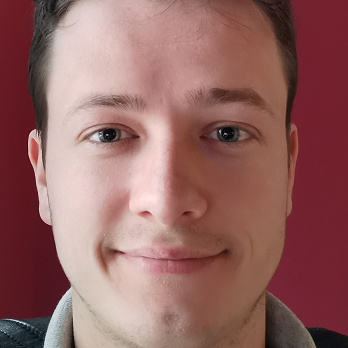
\includegraphics[scale=0.6]{img/eye_section/eye_cropped_face.png}}
        \hspace{8mm}
        \subfigure[Obszar po obcięciu]{\label{fig:eye_crop_after}
\includegraphics[scale=0.6]{img/eye_section/eye_cropped_eyes.png}}
    \end{center}
    \caption{Obcięcie obszaru detekcji oczu zgodnie z dobranymi wcześniej parametrami}
    \label{fig:eye_crop}
\end{figure}

Wprowadzenie takiej modyfikacji pozwoliło odrzucić część błędnie ustalanych obszarów, szczególnie w dolnej części twarzy. Przykład poprawionej detekcji oczu dzięki temu zabiegowi widoczny jest na rysunku \ref{fig:eye_detect_crop}

\begin{figure}[!h]
    \begin{center}
        \subfigure[Wykrywanie oczu bez dodatkowego obcięcia obszaru]{\label{fig:eye_detect_crop_before}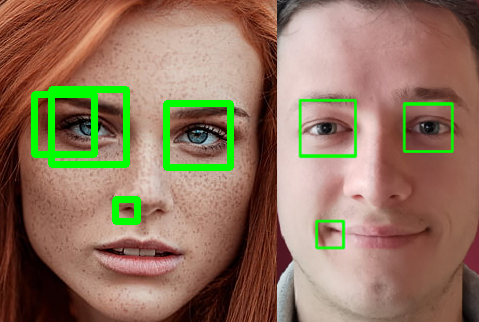
\includegraphics[scale=0.45]{img/eye_section/eye_detect_before_crop_1.png}}
        \hspace{8mm}
        \subfigure[Wykrywanie oczu z dodatkowym obcięciem obszaru]{\label{fig:eye_detect_crop_after}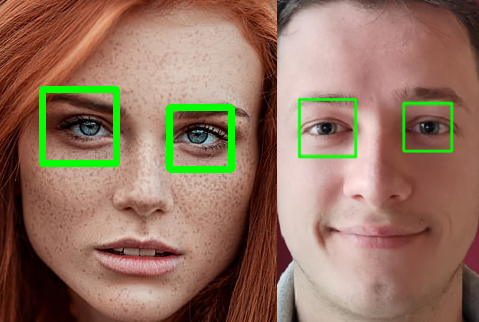
\includegraphics[scale=0.45]{img/eye_section/eye_detect_after_crop_1.png}}
    \end{center}
    \caption{Odrzucenie błędnych rezultatów detekcji oczu po dodatkowym obcięciu obszaru. Źródło pierwszego zdj.:\cite{readheadPortrait2}}
    \label{fig:eye_detect_crop}
\end{figure}


\subsection{Dostosowanie wielkości obszaru facemarków oczu} \label{section:facemark_eye_size}

Dla metody opartej o punkty charakterystyczne twarzy zdecydowałem się dodać pewną tolerancję do obszaru wynikającego jedynie z połączenia tych punktów.
\par
Ustalenie jakie zwiększenie zwracanego regionu da najlepsze rezultaty detekcji oczu odbyło się przez testowe sprawdzenie kombinacji trzech parametrów, które oznaczały wielkość tolerancji z danej strony. W teści przyjmowały one następujące wartości

\begin{itemize}
    \item Góra: z przedziału [0.0, 1.0], będące wielokrotnością $0.1$
    \item Dół: z przedziału [0.0, 1.0], będące wielokrotnością $0.1$
    \item Boki: z przedziału [0.0, 0.5], będące wielokrotnością $0.05$
\end{itemize}

\par

Ze względu na dużą ilość kombinacji ($1331$) nie zostaną podane wyniki, a jedynie wybrana najlepsza kombinacja:
\begin{itemize}
    \item Góra: $0.7$
    \item Dół: $0.5$
    \item Boki: $0.2$
\end{itemize}


\begin{table}[!h]
\label{tab:eye_facemark_size_result}
\centering
\caption{Skuteczność algorytmu detekcji oczu wykorzystując facemarki z dodatkowym zwiększeniem obszaru i bez}
\resizebox{\textwidth}{!}{%
\begin{tabular}{|c|c|c|c|c|c|c|}
\hline
 &
  \textbf{\begin{tabular}[c]{@{}c@{}}Prawidłowe\\ detekcje\end{tabular}} &
  \textbf{\begin{tabular}[c]{@{}c@{}}Perfekcyjne\\ detekcje\end{tabular}} &
  \textbf{\begin{tabular}[c]{@{}c@{}}Częściowo\\ dobre\\ detekcje\end{tabular}} &
  \textbf{\begin{tabular}[c]{@{}c@{}}Złe\\ detekcje\end{tabular}} &
  \textbf{\begin{tabular}[c]{@{}c@{}}Niewykryte\\  oczy otwarte\end{tabular}}  &
 \textbf{\begin{tabular}[c]{@{}c@{}}Niewykryte\\  oczy zamknięte \end{tabular}} \\ \hline \hline
\textbf{\begin{tabular}[c]{@{}c@{}}Facemarki oczu \\ bez zwiększenia obszaru\end{tabular}} &
  142 &
  17 &
  125 &
  14 &
  6 &
  6  \\ \hline

\textbf{\begin{tabular}[c]{@{}c@{}}Facemarki oczu \\ ze zwiększeniem obszaru\end{tabular}} &
  144 &
  142 &
  2 &
  12 &
  6 &
  6  \\ \hline
  
  \hline
\end{tabular}%
}
\end{table}

Zmiany wielkości zwracanego obszaru oczu nie zwiększył znacząco liczby dobrych detekcji. Natomiast największy zysk widoczny jest w perfekcyjnych detekcjach. Dzięki takiemu dostosowaniu udało się osiągnąć prawie $100\%$ wskaźnik perfekcyjnych względem prawidłowych detekcji. Pozwoli to uzyskać lepiej wykryty obszar oczu, co może mieć przełożenie na skuteczność detekcji źrenic.
\newpage

\section{Porównanie algorytmów detekcji oczu}



\subsection{Testowanie na statycznych zdjęciach}

Testowanie detekcji oczu wykorzystując statyczne zdjęcia z datasetu (odrzucone 2, dla których wybrany algorytm nie wykrył prawidłowo twarzy). Znajduje się na nich w sumie 166 oczu do wykrycia, w tym 14 zamkniętych.

\subsubsection{Oczekiwany wynik}
Podobnie jak w przypadku testowania detekcji twarzy na statycznych zdjęciach, tak w przypadku wykrywania oczu akceptowalny obszar był opisany dwoma prostokątami - minimalny i maksymalnym. Przykład takiego oznaczenia widoczny jest na rys. \ref{fig:expected_eyes_region}. Został on dobrany w następujący sposób:
\begin{itemize}
    \item prostokąt wewnętrzny obejmuje jedynie widoczną część gałki ocznej
    \item prostokąt zewnętrzny jest powiększony na boki i w dół o pewną odległość od gałki, a od góry zawiera w sobie również brwi.
\end{itemize}

\begin{figure}[!h]
    \begin{center}
        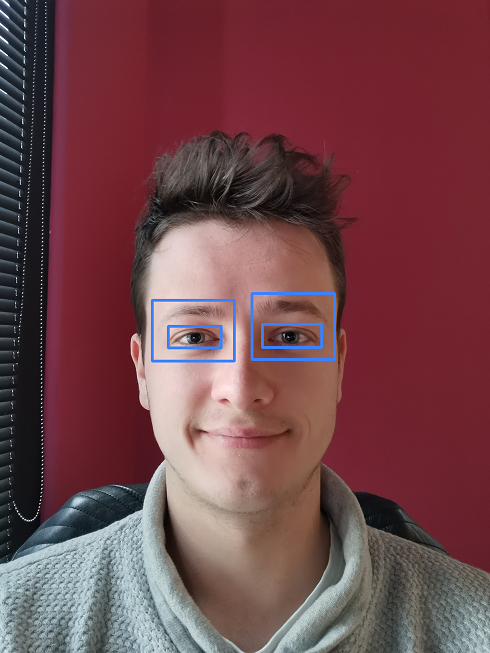
\includegraphics[scale=0.6]{img/pupil_section/expected_eyes_region.png}
        \caption{Przybliżony obszar oczu, który chcę wykrywać}
        \label{fig:expected_eyes_region}
    \end{center}
\end{figure}

\subsection{Warunki testowania}

Oba algorytmy zostaną przetestowane na wykrytych przez algorytm HOG twarzach ze zdjęć 500x500. W tym teście postanowiłem odrzucić już rozdzielczość 300x300, ze względu, że na części z nich osoba jest już bardzo oddalona, co skutkuje bardzo małym rozmiarem oczu. W przypadku korzystania z przedniej kamery telefonu nie będą występowały takie odległości między twarzą, a urządzeniem. Z tego powodu takie warunki nie przyniosłyby znaczących i wartościowych w kontekście pracy dyplomowej wyników. 
\par
Testy zostaną przeprowadzone w przestrzeni barw RGB oraz w skali szarości.

\subsection{Badanie skuteczności detekcji}

Na początku porównywana była skuteczność zaprezentowanych metod. Chociaż w pewien sposób procent detekcji był już przedstawiony podczas dostrajania algorytmów, to tutaj zostały skonfrontowane ze sobą oba algorytmy.
\par
W przypadku metody opartej o facemarki, niewykryte oczy zarówno otwarte jak i zamknięte mogą oznaczać źle określenie położenia lub złą klasyfikacje do jednej z tych grup. Przykładowo oko otwarte mające $EAR$ mniejszy niż ustalony próg klasyfikowane było jako zamknięte, co skutkowało oznaczeniem jako błędna detekcja. 

\begin{table}[!h]
\label{tab:eye_detection_accuracy_result}
\centering
\caption{Skuteczność algorytmów detekcji twarzy}
\resizebox{\textwidth}{!}{%
\begin{tabular}{|c|c|c|c|c|c|c|}
\hline
 &
  \textbf{\begin{tabular}[c]{@{}c@{}}Prawidłowe\\ detekcje\end{tabular}} &
  \textbf{\begin{tabular}[c]{@{}c@{}}Perfekcyjne\\ detekcje\end{tabular}} &
  \textbf{\begin{tabular}[c]{@{}c@{}}Częściowo\\ dobre\\ detekcje\end{tabular}} &
  \textbf{\begin{tabular}[c]{@{}c@{}}Złe\\ detekcje\end{tabular}} &
  \textbf{\begin{tabular}[c]{@{}c@{}}Niewykryte\\  oczy otwarte\end{tabular}}  &
 \textbf{\begin{tabular}[c]{@{}c@{}}Niewykryte\\  oczy zamknięte \end{tabular}} \\ \hline \hline

\textbf{Facemarki oczu RGB} &
  144 &
  142 &
  2 &
  12 &
  6 &
  6  \\ \hline
  
\textbf{\begin{tabular}[c]{@{}c@{}}Facemarki oczu \\ sk. szaro. \end{tabular}} &
  145 &
  140 &
  5 &
  11 &
  1 &
  6  \\ \hline
  
\textbf{Haar RGB} &
  133 &
  95 &
  38 &
  23 &
  9 &
  11  \\ \hline
  
\textbf{Haar sk. szaro.} &
  130 &
  95 &
  35 &
  26 &
  11 &
  7  \\ \hline
  
  \hline
\end{tabular}%
}
\end{table}

Najlepsze wyniki uzyskała metoda oparta na punktach charakterystycznych twarzy w trójkanałowej przestrzeni barw. Udało się jej wykryć średnio  $87\%$ wszystkich oczu. A w przypadku przestrzeni RGB aż $98,6\%$ z nich perfekcyjnie. Ta druga statystyka jest dużo lepsza niż w przypadku metod Haar które uzyskały raptem $57\%$. Ogólnie algorytm wykorzystujący facemarki był lepszy od drugiego o około $10\%$.
\par
Co ciekawe większą liczbę dobrych detekcji metoda oparta o facemarki uzyskała w przypadku obrazów w skali szarości, ale mniej perfekcyjnych. Natomiast, algorytm Haar lepiej poradził sobie w przypadku trójkanałowego zestawu barw, ale wykrywał ona więcej zamkniętych oczu przez co w tej statystyce wypadł gorzej niż w skali szarości. 

\vspace{5mm}

Ważną różnicą w działaniu obu algorytmów jest kształt i rozmiar oznaczanego obszaru. Metoda oparta o klasyfikatory zwraca kwadratowy region, zawierający dużo większą część twarzy niż same oczy. Natomiast facemarki tworzą obszar o kształcie prostokąta o dowolnym stosunku boków i zawierają głównie samą gałkę oczną. Zmniejsza to ilość punktów, które mogą przeszkadzać np. w detekcji źrenic.

\subsubsection{Badanie szybkości detekcji} \label{section:eye_detection_speed_img}


Dla detekcji oczu z użyciem facemarków zostały przedstawione dwa wyniki czasowe - jeden uwzględniający czas wykrycia punktów charakterystycznych, a drugi bez. Związane jest to z faktem, że mimo iż do wykorzystania tej metody niezbędna jest detekcja facemarków, to etap taki i tak będzie wykonany, ponieważ punkty te są używane np. do stwierdzenia mrugnięcia. W przypadku czasów zawierających algorytm punktów charakterystycznych test był przeprowadzony dla dwóch przestrzeni barw. Natomiast, na szybkość przekształcenia facemarków w obszar oka nie wpływa liczba kanałów, ponieważ nie operuje on na pikselach, tylko na zwróconych punktach kartezjańskich. Z tego powodu przedstawiony jest tylko jeden wynik.

\begin{table}[!h]
\label{tab:eye_detect_speed_RGB}
\centering
\caption{Czas przetwarzania algorytmów detekcji twarzy dla obrazów RGB}

\begin{tabular}{|c|c|c|c|}
\hline
 & 
  \textbf{\begin{tabular}[c]{@{}c@{}}Całkowity czas \\ przetwarzania \end{tabular}} &
  \textbf{\begin{tabular}[c]{@{}c@{}}Średni czas\\ przetwarzania \\ pojedynczej iteracji\end{tabular}} &
  \textbf{\begin{tabular}[c]{@{}c@{}}Średni czas\\przetwarzania \\ pojedynczego\\zdjęcia\end{tabular}} \\ \hline\hline
  
\textbf{\begin{tabular}[c]{@{}c@{}}Facemarki oczu RGB\\ (z detekcją facemarków)\end{tabular}} & 
  5,638 s &
  0,281 s &
  0,00361 s    \\ \hline
  
  \textbf{\begin{tabular}[c]{@{}c@{}}Facemarki oczu sk. szaro. \\ (z detekcją facemarków)\end{tabular}} & 
  5,803 s &
  0,290 s &
  0,00372 s    \\ \hline
  
\textbf{\begin{tabular}[c]{@{}c@{}}Facemarki oczu \\ (bez detekcją facemarków)\end{tabular}} & 
  0,024 s &
  0,00122 s &
  0,00000157 s  \\ \hline
  
\textbf{Haar RGB} & 
  26,219 s &
  1,310 s &
  0,0168 s     \\ \hline
  
\textbf{Haar sk. szaro.} & 
  25,830 s &
  1,291 s &
  0,0165 s    \\ \hline
  
  \hline
\end{tabular}%

\end{table}

Wyniki bezdyskusyjnie pokazują dużo większą szybkość detekcji oczu z użyciem facemarków. Nawet biorąc pod uwagę czas wykrycia punktów charakterystycznych metoda ta była ponad $4$ razy szybsza od algorytmu opartego na klasyfikatorach kaskadowych Haar. 
\par
Tworzenia obszarów z punktów charakterystycznych osiągnęło czas rzędu $10^{-5}$, co w porównaniu do pozostałych algorytmów wykorzystywanych w projekcie jest praktycznie zerowy. Tak krótki czas przetwarzania sprawia, że nie będzie on miał żadnego wpływu na ilość klatek na sekundę podczas odbierania obrazu na żywo z kamery.
\par
Przestrzeń barw nie miała znaczącego wpływu na czas detekcji, a wyniki w przypadku trójkanałowych kolorów były porównywalne do skali szarości.

\subsection{Testowanie na obrazie z kamery na żywo}

Detekcja oczu została przetestowana również na obrazie z kamery na żywo. Warunki przeprowadzenia eksperymentu zostały opisane w rozdz. \hyperref[{section:face_detection_test_live}]{\ref{section:face_detection_test_live}}.

\subsubsection{Skuteczność detekcji}

Obserwując na żywo detekcje oczu byłem w stanie wysnuć kilka wniosków na temat badanych algorytmów.

\vspace{4mm}

Przede wszystkim oba działały bardzo stabilnie. Nie występowało nieuzasadnione gubienie obszaru oczu podczas statycznego położenia głowy. 
\par
W metodzie Haar występował problem przy mocnym skręceniu głowy w bok. Zwracany był wtedy często błędny i bardzo powiększony obszar dalszego oka. 
\par
Natomiast detekcja oczu na podstawie facemarków miała problemu z mocno przymkniętymi oczami. Wskaźnik EAR sygnalizował wtedy je jako zamknięte przez co algorytm nie zwracał ich regionu.

\subsubsection{Szybkość detekcji}

Ze względu na praktycznie zerowy obciążenie podczas przekształcania facemarków w obszar twarzy (patrz rozdz. \hyperref[{section:eye_detection_speed_img}]{\ref{section:eye_detection_speed_img}}) wyniki dla facemarków zostały skopiowane z rezultatów uzyskanych przez algorytm Kazemi podczas porównania metod nakładania punktów charakterystycznych na obraz z kamery na żywo  w rozdz. \hyperref[{section:facemark_speed_live}]{\ref{section:facemark_speed_live}}.
\par
Ponownie detekcja twarzy odbywała się przy zastosowaniu algorytmu \textit{HOG} dostarczając obraz RGB.

\begin{table}[!h]
\label{tab:eye_detection_speed_live}
\centering
\caption{Szybkość algorytmów detekcji oczu dla obrazu na żywo z kamery [klatki/s]}
\begin{tabular}{|c|c|c|c|c|c|}
\hline
 \textbf{\begin{tabular}[c]{@{}c@{}}Warunki\end{tabular}} &
  \begin{tabular}[c]{@{}c@{}}1.\end{tabular} &
  \begin{tabular}[c]{@{}c@{}}2.\end{tabular} &
  \begin{tabular}[c]{@{}c@{}}3.\end{tabular} &
  \begin{tabular}[c]{@{}c@{}}4.\end{tabular} &
  \textbf{\begin{tabular}[c]{@{}c@{}}Średnia:\end{tabular}}\\ \hline \hline
\textbf{Haar RGB} &
  11,698 &
  13,600 &
  12,290 &
  12,942 &
  12,632  \\ \hline

\textbf{Haar sk. szaro.} &
  11,956 &
  12,403 &
  12,333 &
  12,472 &
  12,290 \\ \hline
  
\textbf{Znaczniki RGB} &
  15,887 &
  15,941 &
  16,077 &
  16,171 &
  16,019  \\ \hline
  
\textbf{Znaczniki sk. szaro.} &
  15,747 &
  16,146 &
  15,866 &
  16,096 &
  15,963 \\ \hline

  \hline
\end{tabular}%

\end{table}

Test ten pokazał znaczną przewagę szybkościową metody opartej na facemarkach. Klasyfikatory kaskadowe uzyskały około $23\%$ mniejszą liczbę klatek na sekundę.



\subsection{Wybór algorytmu}

Porównanie dwóch algorytmów detekcji oczu bezdyskusyjnie pokazało wyższość metody opartej na facemarkach nad klasyfikatorem kaskadowym Haar. Punkty charakterystyczne uzyskały lepszy procentowo wynik prawidłowych detekcji, a dodatkowo w teście na statycznych zdjęciach prawie wszystkie były perfekcyjne. Próby szybkościowe jednoznacznie wskazały na facemarki, które były $4$ razy szybsze od Haar, a jeśli brać pod uwagę jedynie czas tworzenia obszarów to ponad tysiąckrotnie.
\par
Na podstawie przeprowadzonych testów zostały wybrane facemarki do detekcji oczu i to ten algorytm będzie wykorzystywany w projekcie i pracy dyplomowej.
\newpage

\section{Detekcja źrenic}

W pracy dyplomowej występuje sterowanie aplikacją za pomocą ruch gałek ocznych, w~szczególności analizując położenie źrenic. Mając wykryty obszar oczu (patrz rozdz.~\hyperref[{section:eye_detection}]{\textit{\ref{section:eye_detection}}}) metodami klasycznymi przetwarzania obrazów określane położenie środka źrenicy.

\par

W projekcie zaimplementowane zostały trzy algorytmy do testów i~wybrany jeden, który dawał najlepsze rezultaty.

\subsection{Algorytmy detekcji źrenic}

\subsubsection{Algorytm CDF (Cumulative Distribution Function)}
Algorytm zaimplementowany na podstawie dwóch artykułów o~detekcji źrenic~\cite{IMECSPupilCDFAnalysis}~\cite{EyePupilWebCam}. Opiera się w~głównej mierze na progowaniu za pomocą dystrybuanty. Następnie analizuje najciemniejszy obszar wyznaczany jest środek źrenicy.

\iffalse
\begin{figure}[!h]
    \begin{center}
        \subfigure[Oko skierowane w~prawo]{\label{fig:pupil_cdf_left}
\includegraphics[scale=0.3]{img/pupil_section/pupil_2eyes_left_1.png}}
        \hspace{3mm}
        \subfigure[Oko skierowane na wprost]{\label{fig:pupil_cdf_center}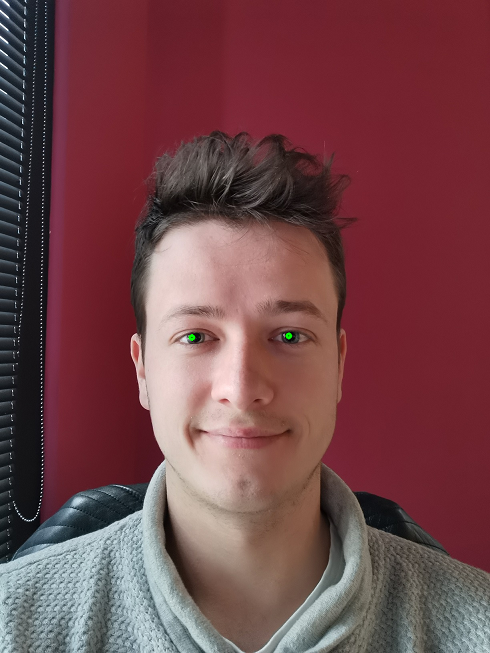
\includegraphics[scale=0.3]{img/pupil_section/pupil_2eyes_center_1.png}}
        \hspace{3mm}
        \subfigure[Oko skierowane w~lewo]{\label{fig:pupil_cdf_right}
\includegraphics[scale=0.3]{img/pupil_section/pupil_2eyes_right_1.png}}
    \end{center}
    \caption{Rezultat wykrywania źrenic metodą CDF}
    \label{fig:cdf_results}
\end{figure}
\fi

\paragraph{Kroki algorytmu}

\begin{itemize}
    \item Za pomocą progowania z~użyciem dystrybuanty tworzony jest obraz binarny.\\
    \begin{align}
        CDF(r) = \sum_{w=0}^{r} p(w)
    \end{align}
    
    Gdzie \textit{p(w)} to prawdopodobieństwo znalezienia punktu o~jasności równej \textit{w} - określone przy pomocy dystrybuanty.
    
    \begin{align}
        I`(x, y) = 
        \begin{cases}
            255, &  CDF(I(x, y)) < \textit{a}\\
            0,   &  wpp
        \end{cases}
    \end{align} 
    
    Gdzie \textit{I} to jasność piksela, natomiast \textit{a} to ustalony próg

    \item Na uzyskany obraz binarny nakładana jest operacja morfologiczna erozji (filtr minimalny), celem usunięcia pojedynczych ciemnych pikseli
    
    \item Następnie znajdowany jest najciemniejszy piksel na oryginalnym obrazie wśród tych, które mają wartość~255 (są białe) na obrazie binarnym
    
    \item Obliczana jest średnia jasność pikseli w~kwadracie~10x10 wokół wybranego najciemniejszego punktu
    
    \item Nakładana jest erozja na obszarze~15x15 wokół wybranego punktu
    
    \item Na tym obszarze stosowane jest progowanie na podstawie wartości
    
    \begin{align}
        I`(x, y) = 
        \begin{cases}
            255, &  I(x, y) < I_{AVG}\\
            0,   &  wp.p.
        \end{cases}
    \end{align}
    
    Gdzie \textit{$I_{AVG}$} to średnia jasność obszaru obliczona wcześniej
    
    \item Szukanym punktem źrenicy jest środek ciężkości białych punktów na uzyskanym binarnym obrazie

\end{itemize}

\iffalse
\begin{figure}[!h]
    \begin{center}
        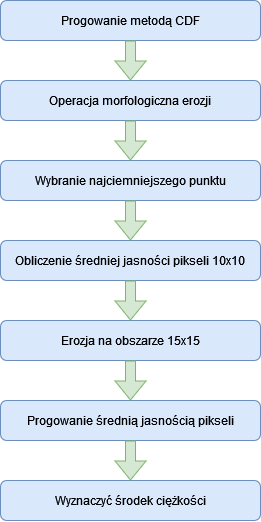
\includegraphics[scale=0.35]{img/pupil_section/CDF_Diagram.png}
        \caption{Kroki algorytmu metodą CDF}
        \label{fig:cdf_diagram}
    \end{center}
\end{figure}
\fi

\paragraph{Wynik kolejnych kroków algorytmu}
Na \hyperref[{fig:cdf_steps}]{\textit{rys.~\ref{fig:cdf_steps}}} przedstawiony jest rezultat kolejnych etapów wykrywania źrenic przy pomocy metody \textit{CDF} na przykładowym zdjęciu oka.

\begin{figure}[!h]
    \begin{center}
        \subfigure[Obszar oka w~skali szarości]{\label{fig:cdf_gray}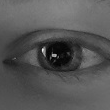
\includegraphics[scale=0.50]{img/pupil_section/CDF_steps/CDF_gray_eye.png}}
        \hspace{8mm}
        \subfigure[Wynik progowania CDF]{\label{fig:cdf_binary}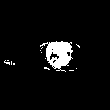
\includegraphics[scale=0.50]{img/pupil_section/CDF_steps/CDF_binary_eye_after_CDF.png}}
        \hspace{8mm}
        \subfigure[Wynik erozji]{\label{fig:cdf_erode}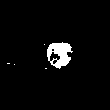
\includegraphics[scale=0.50]{img/pupil_section/CDF_steps/CDF_binary_eye_after_erode.png}}
        
        \hfill
        
        \subfigure[Najciemniejszy punkt]{\label{fig:cdf_darkest}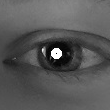
\includegraphics[scale=0.50]{img/pupil_section/CDF_steps/CDF_darkest_pixel.png}}
        \hspace{8mm}
        \subfigure[Obszar 10x10, w~którym obliczana jest średnia jasność]{\label{fig:cdf_avgIntens}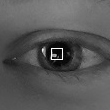
\includegraphics[scale=0.50]{img/pupil_section/CDF_steps/CDF_avgIntensity_region.png}}
        \hspace{8mm}
        \subfigure[Wynik erozji]{\label{fig:cdf_eroded}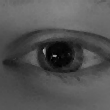
\includegraphics[scale=0.50]{img/pupil_section/CDF_steps/cdf_eroded_eye.png}}
        
        \hfill
        
        \subfigure[Obszar 15x15, który poddawany jest progowaniu]{\label{fig:cdf_pmi}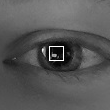
\includegraphics[scale=0.50]{img/pupil_section/CDF_steps/CDF_pmi.png}}
        \hspace{8mm}
        \subfigure[Progowanie średnią jasnością pikseli]{\label{fig:cdf_threshold}
\includegraphics[scale=3.65]{img/pupil_section/CDF_steps/CDF_threshold_pmi.png}}
        \hspace{8mm}
         \subfigure[Wykryte położenie źrenicy]{\label{fig:cdf_pupil_detected}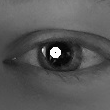
\includegraphics[scale=0.50]{img/pupil_section/CDF_steps/CDF_pupil_detected.png}}

        
    \end{center}
    \caption{Kolejne etapy wykrywania źrenic metodą CDF}
    \label{fig:cdf_steps}
\end{figure}









\subsubsection{Algorytm PF (Projection Function)}

Algorytm po raz pierwszy opisany w~artykule zatytułowanym \textit{Projection Functions for Eye Detection} \cite{projection_function} z~2004 roku. Jest oparty na rzutowaniu jasności pikseli na składowe poziome i~pionowe. Do obliczenia tych wartości wykorzystuje się funkcje projekcji, która może przyjmować różne postaci - z~czego trzy zostały opisane w~tej pracy dyplomowej. Największe różnice wartości oznaczają szybkie zmiany jasności, które mogą być konturami oka.~\cite{EyePupilWebCam}

\paragraph{Funkcja projekcji}

Funkcja projekcji służąca do rzutowania jasności rzędów i~kolumn może przyjmować różne formy. Najczęściej stosowana jest funkcja całkowa, jednak ze względu na swoje niedociągnięcia i~kłopoty z~wykrywaniem wariancji powstały także inne algorytmy. Trzy różne funkcje opisane są poniżej.

\subparagraph{Funkcja całkowa} Wylicza się za jej pomocą średnią jasność pikseli w~danym rzędzie lub kolumnie. w~teorii jest to całka:
\begin{align}
    {IPF_h}(y) = \frac{1}{{x_b}-{x_a}}\int_{x_a}^{x_b} I(x,y) \, \mathrm{d}x
\end{align}
\begin{align}
    {IPF_v}(x) = \frac{1}{{y_b}-{y_a}}\int_{y_a}^{y_b} I(x,y) \, \mathrm{d}y
\end{align}

Ale w~praktyce degeneruje się do funkcji sumy:

\begin{align}
    {IPF_h}(y)=\frac{1}{{x_b}-{x_a}}\sum_{x={x_a}}^{{x_b}} I(x,y)
\end{align}
\begin{align}
    {IPF_v}(x)=\frac{1}{{y_b}-{y_a}}\sum_{y={y_a}}^{{y_b}} I(x,y)
\end{align}

\subparagraph{Funkcja wariancji} Średnia różnica między jasnością danego piksela, a~wyliczonego \textit{IPF} danego rzędu lub kolumny

\begin{align}
    {VPF_h}(y)=\frac{1}{{x_b}-{x_a}}\sum_{x={x_a}}^{{x_b}} (I(x,y) - {IPF_h(y)})
\end{align}
\begin{align}
    {VPF_v}(x)=\frac{1}{{y_b}-{y_a}}\sum_{y={y_a}}^{{y_b}} (I(x,y) - {IPF_v(x)})
\end{align}

Chociaż we wskazanym wyżej artykule funkcja ta występuje w~przedstawionej formie to spotykane są również postacie z~różnicą kwadratową oraz z~pierwiastkami z~obliczonej wartości. 

\subparagraph{Funkcja ogólna} Parametryzowana suma wyliczonych wartości \textit{IPF} i~\textit{VPF}.

\begin{align}
    {GPF_h}(y)=(1-\alpha) * {IPF_h(y)} + \alpha * {VPF_h(y)}
\end{align}
\begin{align}
    {GPF_v}(x)=(1-\alpha) * {IPF_v(x)} + \alpha * {VPF_v(x)} 
\end{align}

Autorzy tej metody zalecają parametr $\alpha = 0.6$ jako dający najlepsze rezultaty.

\paragraph{Kroki algorytmu}

\begin{itemize}
    \item Dla każdego rzędu i~kolumny obliczana jest wartość funkcji projekcji
    \item Dla wyliczonych funkcji projekcji określana jest wartość pochodnej w~każdym rzędzie i~kolumnie
    \item Wybierane są dwa ekstrema dla poziomego i~pionowego wymiaru
    \item Przecięcie wybranych kolumn i~rzędów tworzy prostokąt, którego śreodek jest poszukiwany punkt na źrenicy 
\end{itemize}

\paragraph{Wynik kolejnych kroków algorytmu}
Na \hyperref[{fig:pf_steps}]{\textit{rys.~\ref{fig:pf_steps}}} przedstawiony jest rezultat kolejnych etapów wykrywania źrenic przy pomocy metody \textit{PF} na przykładowym zdjęciu oka.

\begin{figure}[!h]
    \begin{center}
        \subfigure[Obszar oka w~skali szarości]{\label{fig:pf_gray_eye}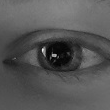
\includegraphics[scale=0.50]{img/pupil_section/PF_steps/PF_gray_eye.png}}
        \hspace{8mm}
        \subfigure[Pionowe wartości projekcji]{\label{fig:pf_x_projection}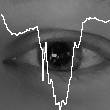
\includegraphics[scale=0.50]{img/pupil_section/PF_steps/PF_x_projection.png}}
        \hspace{8mm}
        \subfigure[Poziome wartości projekcji]{\label{fig:pf_y_projection}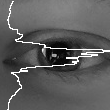
\includegraphics[scale=0.50]{img/pupil_section/PF_steps/PF_y_projection.png}}
        
        \hfill
        
        \subfigure[Pionowe wartości pochodnej]{\label{fig:pf_x_derviatives}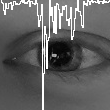
\includegraphics[scale=0.5]{img/pupil_section/PF_steps/PF_x_derivaties.png}}
        \hspace{8mm}
        \subfigure[Poziome wartości pochodnej]{\label{fig:pf_y_derviatives}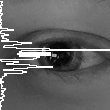
\includegraphics[scale=0.5]{img/pupil_section/PF_steps/PF_y_derivatives.png}}
        \hspace{8mm}
        \subfigure[Pionowe ekstrema]{\label{fig:pf_x_extremum}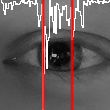
\includegraphics[scale=0.50]{img/pupil_section/PF_steps/PF_x_extremum.png}}
        
        \hfill
        
        \subfigure[Poziome ekstrema]{\label{fig:pf_y_extemum}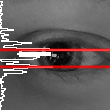
\includegraphics[scale=0.5]{img/pupil_section/PF_steps/PF_y_extremum.png}}
        \hspace{8mm}
        \subfigure[Środek wybranego obszaru]{\label{fig:pf_lines_intersection}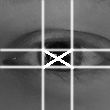
\includegraphics[scale=0.65]{img/pupil_section/PF_steps/PF_lines_intersection.png}}
        \hspace{8mm}
        \subfigure[Wykryte położenie źrenicy]{\label{fig:pf_pupil_detected}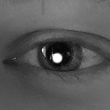
\includegraphics[scale=0.50]{img/pupil_section/PF_steps/PF_pupil_detected.png}}
        
    \end{center}
    \caption{Kolejne etapy wykrywania źrenic metodą PF}
    \label{fig:pf_steps}
\end{figure}






\subsubsection{Algorytm EA (Edge Analysis)}

Algorytm detekcji źrenic \cite{EyePupilWebCam} opierający się na wykryciu i~analizie krawędzi. w~teorii krawędzie najbardziej pionowe i~poziome na zdjęciu powinny należeć do tęczówki i~źrenicy.

\paragraph{Kroki algorytmu}

\begin{itemize}
    \item Dla obszaru oka w~skali szarości nakładany jest filtr rozmywający, np. Gaussa. Pozwala to pozbyć się drobnych szumów i~wygładzić obraz.
    \item Wykrywane są krawędzie i~tworzony obraz binarny. Można zastosować np. algorytm Canny, który jest jedną z~najpopularniejszych metod detekcji krawędzi
    \item Wybierane są dwa rzędy i~dwie kolumny z~największą liczbą punktów o~wartości~255 (białe piksele na obrazie binarnym)
    \item Przecięcie wybranych rzędów i~kolumn tworzy prostokąt, którego środek jest poszukiwany punkt na źrenicy
\end{itemize}

\paragraph{Wynik kolejnych kroków algorytmu}
Na \hyperref[{fig:ea_steps}]{\textit{rys.~\ref{fig:ea_steps}}} przedstawiony jest rezultat kolejnych etapów wykrywania źrenic przy pomocy metody \textit{EA} na przykładowym zdjęciu oka.

\begin{figure}[!h]
    \begin{center}
        \subfigure[Obszar oka w~skali szarości]{\label{fig:ea_gray_eye}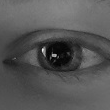
\includegraphics[scale=0.50]{img/pupil_section/EA_steps/EA_gray_eye.png}}
        \hspace{8mm}
        \subfigure[Rozmycie filtrem Gaussa]{\label{fig:ea_gaussian}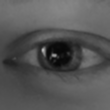
\includegraphics[scale=0.50]{img/pupil_section/EA_steps/EA_gaussian.png}}
        \hspace{8mm}
        \subfigure[Detekcja krawędzi metodą Canny]{\label{fig:ea_canny}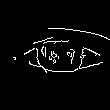
\includegraphics[scale=0.50]{img/pupil_section/EA_steps/EA_canny.png}}
        
        \hfill
        
        \subfigure[Najliczniejsze rzędy i~kolumny]{\label{fig:ea_canny_lines}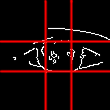
\includegraphics[scale=0.65]{img/pupil_section/EA_steps/EA_canny_lines.png}}
        \hspace{8mm}
        \subfigure[Środek wybranego obszaru]{\label{fig:ea_lines_intersection}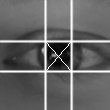
\includegraphics[scale=0.5]{img/pupil_section/EA_steps/EA_lines_intersection.png}}
        \hspace{8mm}
        \subfigure[Wykryte położenie źrenicy]{\label{fig:ea_pupil_detected}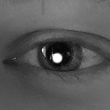
\includegraphics[scale=0.50]{img/pupil_section/EA_steps/EA_pupil_detected.png}}
    \end{center}
    \caption{Kolejne etapy wykrywania źrenic metodą EA}
    \label{fig:ea_steps}
\end{figure}
\newpage
\section{Porównanie detekcji źrenic}

Podobnie jak w pozostałych detekcjach, tak i w przypadku wykrywania źrenic algorytmy zostały porównane i wybrany jeden - najlepszy.

\subsection{Testowanie na statycznych zdjęciach}

\subsubsection{Oczekiwany wynik}

Oczekiwany rezultat detekcji źrenic został opisany dwoma parametrami:
\begin{itemize}
    \item \textbf{Środek źrenicy} - punkt kartezjański
    \item \textbf{Obszar tęczówki} - prostokątny obszar 
\end{itemize}

Przykładowe zdjęcie oka wraz z naniesionymi elementami pokazane jest na rysunku \ref{fig:expected_pupil}.


\begin{figure}[!h]
    \begin{center}
        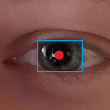
\includegraphics[scale=1.0]{img/pupil_section/pupil_expected.png}
        \caption{Przybliżona lokalizacja źrenicy i obszar tęczówki, które są oczekiwanym wynikiem algorytmu.}
        \label{fig:expected_pupil}
    \end{center}
\end{figure}

\subsubsection{Zbierane dane}

Podczas testów zbierane były następujące dane:

\begin{itemize}
    \item \textbf{W obszarze tęczówki} - ilość wykrytych punktów znajdujących się wewnątrz tęczówki oka
    \item \textbf{Poza obszarem tęczówki} - ilość wykrytych punktów znajdujących się poza tęczówką oka
    \item \textbf{Średni błąd} - średni błąd ze wszystkich detekcji (patrz Uwaga 1.)
    \item \textbf{Błąd <= 0.1} - ilość detekcji z~błędem nie większym niż $10\%$
    \item \textbf{Błąd <= 0.05} - ilość detekcji z~błędem nie większym niż $5\%$
\end{itemize}

\par

\textit{Uwaga 1.} Błąd (wykrycia punktu kartezjańskiego źrenicy) dla danego zdjęcia obliczany był następującym wzorem

\begin{align}
    b(P_1, P_2) = \frac{dist(P_1, P_2)}{hypot(w, h)} * 100\%
\end{align}

Gdzie:

\begin{itemize}
    \item \textbf{P\textsubscript{1}} - wykryty punkt
    \item \textbf{P\textsubscript{2}} - oczekiwany środek źrenicy
    \item \textbf{dist} - odległość między punktami (euklidesowa)
    \item \textbf{hypot} - przeciwprostokątna dla podanych przyprostokątnych (w przypadku regionu oka jest to przekątna)
    \item \textbf{w}, \textbf{h} - szerokość i~wysokość regionu oka
\end{itemize}



\subsubsection{Wybór funkcji projekcji}

Ze względu, że metoda PF może wykorzystywać różne funkcje projekcji do swojego działania konieczne było wyznaczenie i~wybranie najlepszej opcji. Badanie skuteczności przeprowadzone było dla następującego zestawu funkcji:

\begin{itemize}
    \item Całkowa
    \item Wariancja kwadratowa
    \item Wariancja pierwiastkowa
    \item Wariancja liniowa
    \item Ogólna z~wariancją kwadratową
    \item Ogólna z~wariancją pierwiastkową
    \item Ogólna z~wariancją liniową
\end{itemize}

W~przypadku funkcji ogólnej dodatkowo zostało przeprowadzone przeszukiwanie celem ustalenia najlepszego współczynnika $\alpha$ dla poszczególnych opcji. Badana była wielkość tego parametru w~przedziale $[0.01, 0.99]$ ze skokiem $0.01$ (wykluczono wartości $0.00$ oraz $1.00$, ponieważ odpowiadają one odpowiednio funkcji całkowej i~funkcji wariancji).

\par

Finalnie najlepsze w~poszczególnych wariantach okazały się następujące wartości współczynnika $\alpha$:

\begin{itemize}
    \item Ogólna z~wariancją kwadratową: $0.99$
    \item Ogólna z~wariancją pierwiastkową: $0.01$
    \item Ogólna z~wariancją liniową: $0.31$
\end{itemize}

W przypadku funkcji ogólnej z~wariancją kwadratową najlepszy rezultat dał parametr $\alpha=0.99$, co w~przybliżeniu degeneruje ją do wariancji kwadratowej. Natomiast w~przypadku pierwiastkowej ($\alpha=0.01$) do funkcji całkowej. Potwierdzają to również wyniki w~tabeli~\ref{tab:eye_pupil_projection_accuracy_result}, gdzie opisane przypadki osiągają takie same lub zbliżone rezultaty.

\begin{table}[!h]

\centering
\caption{Skuteczność algorytmu PF zależnie od funkcji projekcji na zbiorze danych}
\label{tab:eye_pupil_projection_accuracy_result}
\begin{tabular}{|c|c|c|c|c|c|}
\hline
 &
  \textbf{\begin{tabular}[c]{@{}c@{}}W obszarze \\ tęczówki \end{tabular}} &
  \textbf{\begin{tabular}[c]{@{}c@{}}Poza obszarem \\ tęczówki \end{tabular}} &
  \textbf{\begin{tabular}[c]{@{}c@{}}Średni \\ błąd\end{tabular}} &
  \textbf{\begin{tabular}[c]{@{}c@{}}Błąd \\ <= 0.1\end{tabular}} &
  \textbf{\begin{tabular}[c]{@{}c@{}}Błąd \\ <= 0.5\end{tabular}}
  \\ \hline \hline

\textbf{Całkowa} &
  85 &
  51 &
  14,35\% &
  53 &
  26  \\ \hline
  
\textbf{Wariancji, kwadratowa} &
  98 &
  38 &
  13,51\% &
  60 &
  27 
  \\ \hline
  
\textbf{Wariancji, pierwiastkowa} &
  79 &
  57 &
  14,66\% &
  47 &
  29  \\ \hline
  
  \textbf{Wariancji, liniowa} &
  51 &
  85 &
  23,12\% &
  24 &
  4  \\ \hline
  
  \textbf{Ogólna, kwadratowa} &
  98 &
  38 &
  13,51\% &
  60 &
  27 
  \\ \hline
  
\textbf{Ogólna, pierwiastkowa} &
  85 &
  51 &
  14,27\% &
  53 &
  26  \\ \hline
  
  \textbf{Ogólna, liniowa} &
  86 &
  50 &
  14,17\% &
  53 &
  26  \\ \hline
  
  \hline
\end{tabular}%
\end{table}

Najlepszą skuteczność wykazały funkcje wariancji kwadratowej oraz ogólna kwadratowa. Wykryły one najwięcej punktów wewnątrz tęczówki - $72\%$ oraz uzyskały najmniejszy średni błąd - $13.51\%$. Ze względu na opisaną wyżej degradacje, której przyczyną jest współczynnik $\alpha$ z~tej pary wybrana została funkcja wariancji, która musi wykonać mniej obliczeń w~czasie swojego działania. Dlatego ta wersja funkcji była wykorzystywana w~dalszej części badań.

\subsubsection{Badanie skuteczności detekcji}






\begin{table}[!h]
\label{tab:eye_pupil_detection_accuracy_result}
\centering
\caption{Skuteczność algorytmów detekcji źrenic na zbiorze danych}
\begin{tabular}{|c|c|c|c|c|c|}
\hline
 &
  \textbf{\begin{tabular}[c]{@{}c@{}}W obszarze \\ tęczówki \end{tabular}} &
  \textbf{\begin{tabular}[c]{@{}c@{}}Poza obszarem \\ tęczówki \end{tabular}} &
  \textbf{\begin{tabular}[c]{@{}c@{}}Średni \\ błąd\end{tabular}} &
  \textbf{\begin{tabular}[c]{@{}c@{}}Błąd \\ <= 0.1\end{tabular}} &
  \textbf{\begin{tabular}[c]{@{}c@{}}Błąd \\ <= 0.5\end{tabular}}
  \\ \hline \hline

\textbf{CDF} &
  113 &
  23 &
  10,72\% &
  87 &
  54  \\ \hline
  
\textbf{PF} &
  98 &
  38 &
  13,51\% &
  60 &
  27 
  \\ \hline
  
\textbf{EA} &
  68 &
  68 &
  19,68\% &
  42 &
  14  \\ \hline
  
  \hline
\end{tabular}%
\end{table}


W przypadku progowania przy pomocy dystrybuanty na prawidłową detekcje wpływ miała jakość wycinka zdjęcia podawanego na wejście metody. W~przypadku gdy duża była jego ostrość, a~oko zajmowało subiektywnie duży obszar to algorytm radził sobie bardzo dobrze. Metoda uzyskiwała dobre wyniki zarówno w~przypadku gdy tęczówka oka była ciemna, jak i~jasna. Negatywny wpływ na skuteczność detekcji miało występowanie na wycinku zdjęcia brwi, a~w~szczególności gdy były one w~ciemnym odcieniu lub nałożony był na nie mocny makijaż. Podobnie intensywna barwa rzęs skutkowała obniżeniem dokładności wskazywania lokalizacji źrenicy. Lepsze rezultaty metoda uzyskiwała gdy na wycinku znajdowała się tylko i~wyłącznie gałka oczna. W~przypadku gdy źrenica miała jasny odcień wynikający np. z~dużego natężenia padającego światła to uzyskiwane rezultaty nie były zadowalające. Jeśli algorytmowi udało się wskazać punkt należący do tęczówki, to w~większości przypadków wynikiem był jej środek oraz źrenica. W~ogólności, skuteczność tej metody opierała się w~dużej mierze na występowaniu ciemnych punktów innych niż tęczówka i~źrenica.

\par

Metoda projekcji lepsze rezultaty detekcji wykazywała na obszarach oczu o~małym kontraście i~ostrości. Gorsza jakość zdjęć miała pozytywny wpływ na jej działanie. Częstym zjawiskiem było wskazanie tylko jednej składowej poprawnie - poziomej lub pionowej. Algorytm ten w~części przypadków wskazywał rzęsy zamiast źrenic. Prawidłowe detekcje występowały przy bardzo wyraźnych przejściach między białą częścią oka, a~tęczówką. Jeśli region źrenicy był ciemniejszy niż reszta obszaru oka to detekcja uzyskiwała lepsze rezultaty. Występowanie ramek okularów przeszkadzało w~prawidłowym wskazaniu szukanego punktu.

\par

Analiza krawędzi całkowicie nie radziła sobie z~detekcją w~przypadku gdy występowało dużo wyraźnych konturów innych niż tęczówka lub źrenica. Dobre rezultaty osiągane były jeśli obszar oka był jasny i~naświetlony. W~przeciwieństwie do projekcji metoda ta lepiej radziła sobie przy wycinkach dobrej jakości i~o dużej ostrości. Porównując ten algorytm do dwóch pozostałych jego zachowanie wydawało się dużo bardziej losowe, ponieważ w~wielu przypadkach trudno było wskazać powody zwróconej złej lokalizacji. Wyniki procentowe jak i~subiektywne odczucia wskazują jednoznacznie, że metoda oparta na analizie krawędzi radziła sobie znacznie najgorzej.





\subsubsection{Badanie szybkości detekcji} \label{section:test_pupil_speed_img}

\begin{table}[!h]
\label{tab:eye_pupil_speed}
\centering
\caption{Czas przetwarzania algorytmów detekcji źrenic na zbiorze danych}

\begin{tabular}{|c|c|c|c|}
\hline
 & 
  \textbf{\begin{tabular}[c]{@{}c@{}}Całkowity czas \\ przetwarzania \end{tabular}} &
  \textbf{\begin{tabular}[c]{@{}c@{}}Średni czas\\ przetwarzania \\ pojedynczej iteracji\end{tabular}} &
  \textbf{\begin{tabular}[c]{@{}c@{}}Średni czas\\przetwarzania \\ pojedynczego\\zdjęcia\end{tabular}} \\ \hline\hline
  
\textbf{PF} & 
  0,272 s &
  0,00272 s &
  0,00002001 s    \\ \hline
  
\textbf{EA} & 
  0,765 s &
  0,00765 s &
  0,00005627 s  \\ \hline
  
\textbf{CDF} & 
  0,637 s &
  0,00637 s &
  0,00004684 s \\ \hline

  \hline
\end{tabular}%

\end{table}

Najszybszym okazał się algorytm oparty na funkcji projekcji. Przetworzenie jednego wycinka oka zajęło mu średnio $2.0*10^{-5}s$. Dwukrotnie dłużej trwało wykonanie metody z~użyciem progowania opartego o~dystrybuantę. Najwolniej natomiast działała analiza krawędzi uzyskując czas $5.6*10^{-5}$.

\par

Wyniki zdają się oddawać naturę poszczególnych metod, ponieważ projekcja wymaga maksymalnie dwóch przejść całej macierzy obrazu. Natomiast algorytm oparty na analizie krawędzi wykorzystuje filtry oraz metodę Canny, dlatego ma największą złożoność czasową.

\par

Wszystkie metody są bardzo szybkie (rząd wielkości $10^{-5}s$) i~nawet najwolniejsza z~nich mogłaby być wykonana prawie 18 tyś. razy na sekundę. Przekłada się to na zerowe obciążenie całej aplikacji, która wykrywając jedynie twarz osiąga raptem $16$ klatek na sekundę dla barw RGB (rozdział~\ref{section:face_speed_live}). Z~tego powodu podczas wyboru najlepszego algorytmu detekcji źrenic nie była brana pod uwagę szybkość poszczególnych metod, a~jedynie ich skuteczność.




\subsection{Testowanie na obrazie z~kamery}

Przetestowanie skuteczności detekcji na obrazie z~kamery i~przedstawienie ich w~postaci liczbowej byłoby bardzo trudne. Z~tego powodu algorytm został przebadany poprzez obserwacje zachowania detekcji na podglądzie na żywo. Testy były przeprowadzone w~takich samych warunkach jak pozostałe elementy systemu. Wyniki są subiektywnym odczuciem autora projektu i~przedstawione w~formie opisowej. 

\par

Ze względu na wyniki szybkościowe detekcji źrenic (rozdział~\ref{section:test_pupil_speed_img}), które jednoznacznie wykazały marginalny czas przetwarzania wszystkich algorytmów, testy czasowe na obrazie z~kamery na żywo zostały uznane za niepotrzebne i~pominięte.

\subsubsection{Badanie skuteczność detekcji}

Podobnie jak w~testach przeprowadzonych na statycznych zdjęciach algorytm CDF uzyskał subiektywnie najlepsze rezultaty. We wszystkich scenariuszach sprawdził się wystarczająco. Nawet w~momencie gdy nie wykrywał dobrze środka źrenicy to wskazania znajdowały się w~obszarze tęczówki. Pracował stabilnie zarówno w~centralnym położeniu oka jak i~przy wzroku zwróconym w~bok. 

\par 

Algorytm PF radził sobie dobrze tylko połowicznie. Najlepsze rezultaty osiągnął w~przypadku światła padającego zza użytkownika. Wtedy zarówno centralne jak i~boczne położenie był prawidłowo wykrywane. W~pozostałych badaniach dobre wyniki osiągał gdy oczy był skierowane w~bok, a~w~przypadku spojrzenia wprost przed siebie lokalizacja podawana była chaotycznie. Test w~ciemnym pomieszczeniu potwierdził, że metoda dobrze radzi sobie przy małym kontraście i~jasności. 

\par

Analiza krawędzi w~przypadku obrazu na żywo w~ogóle się nie sprawdziła. W~żadnych warunkach detekcja nie była wystarczająca na potrzeby pracy dyplomowej. Przez większość czasu zwracaną lokalizacją były rogi obszaru oczu.


 

\subsection{Wybór algorytmu detekcji źrenic}

Najskuteczniejsza okazała się metoda oparta na progowaniu z~użyciem dystrybuanty. W~teście na zbiorze danych~$83\%$ wykrytych punktów znajdowało się wewnątrz tęczówki. Subiektywnie, najlepsze i~wystarczające rezultaty uzyskała również w~badaniu obrazu na żywo z~kamery.

\par

Szybkość wszystkich algorytmów stała na tak wysokim i~marginalnym poziomie, że nie była brana jako czynnik wpływający na wybór algorytmu.

\par

Z powodu wykrywalności źrenic rozwiązanie CDF zostało wybrane jako najlepsze i podstawowe w~projekcie.
\newpage

\section{Detekcja mrugania}

Celem stwierdzenia czy wystąpiło mrugniecie zostało zaimplementowane proste rozwiązanie polegające na analizie określonej ilości klatek wstecz. Wykorzystywany jest fakt czy w~danej klatce oczy były zamknięte czy otwarte i~zmianę tego stanu system informuje o~ewentualnym wystąpieniu zdarzenia. 

\subsection{Algorytm detekcji mrugania}

\begin{enumerate}
    \item Utworzenie tablicy $T$ przechowującej $a$ wartości typu prawda/fałsz oznaczających czy oczy były zamknięte czy otwarte w~$a$ ostatnich klatkach obrazu.
    \item Usunięcie najstarszej wartości z~tablicy $T$ jeśli jest pełna
    \item Dodanie do tablicy $T$ nowej flagi zamkniętych oczu w~danej klatce
    \item Analiza zawartości tabeli $T$. Jeśli wszystkie pola mają taką samą wartość to ustalenie stanu $S_{i}$ na tę wartość i~porównanie z~poprzednim stanem~$S_{i-1}$:
        \begin{itemize}
            \item Jeśli $S_{i}$ jest inny niż $S_{i-1}$ i~stan $S_{i}$ oznacza oczy zamknięte to wystąpiło mrugnięcie
        \end{itemize}
    \item Powrót do punktu 3
\end{enumerate}

\vspace{3mm}

\textit{Uwaga 1.} Parametr $a$ oznacza ile klatek z~rzędu musi występować dany stan oka by uznać go za wiarygodny (służy odrzuceniu pojedynczych błędnych wskazań i~szumów).

\par

\textit{Uwaga 2.} Stan o~wartości prawda oznacza oczy zamknięte.



\subsection{Testowania detekcji mrugania na obrazie na żywo z~kamery} \label{section:test_eye_blink}

Przeprowadzone zostały testy detekcji ruchu oczu na obrazie na żywo. w~każdych warunkach zostały wykonane trzy testy powtórzone dwukrotnie:

\begin{itemize}
    \item mrugnięcie lewym okiem
    \item mrugnięcie prawym okiem
    \item mrugnięcie oboma oczami na raz
\end{itemize}

Poszczególne czynności w~ramach jednego testu wykonane był 10 razy. 

\begin{table}[!h]
\label{tab:eye_blink_accuracy}
\centering
\caption{Skuteczność wykrywania mrugania na obrazie na żywo z kamery}
\begin{tabular}{|c|c|c|c|c|}
\hline
 \textbf{\begin{tabular}[c]{@{}c@{}}Warunki\end{tabular}} &
  \begin{tabular}[c]{@{}c@{}}1.\end{tabular} &
  \begin{tabular}[c]{@{}c@{}}2.\end{tabular} &
  \begin{tabular}[c]{@{}c@{}}3.\end{tabular} &
  \begin{tabular}[c]{@{}c@{}}4.\end{tabular} \\ \hline \hline
\textbf{Lewym okiem} &
  9 &
  10 &
  10 &
  9 \\ \hline

\textbf{Prawym okiem} &
  10 &
  10 &
  8.5 &
  7 \\ \hline
  
\textbf{Oboma oczami} &
  10 &
  10 &
  10 &
  10 \\ \hline
  
  \hline
\end{tabular}%

\end{table}

Skuteczność detekcji mrugania okazała się bardzo dobra, lepsza niż oczekiwana. w~przypadku testu gdy czynność została wykonana oboma oczami na raz została wykryta ona za każdym razem. w~pozostałych przypadkach osiągała wynik na poziomie średnio~$92\%$ skuteczności. Takie rezultaty wydają się być całkowicie wystarczające i~zadowalające z~perspektywy pracy dyplomowej. 
\newpage

\section{Detekcja ruchu gałek ocznych}

Do detekcji ruchu gałek ocznych wykorzystywany jest identyczny mechanizm jak w~przypadku wykrywania mrugania. Analizowane są położenia źrenic w~określonej ilości klatek obrazu, a~na~ich podstawie zgłaszana jest ewentualna zmiana położenia oczu, a~w~konsekwencji ich ruch. 

\subsection{Algorytm detekcji ruchu oczu}

\begin{enumerate}
    \item Utworzenie tablicy $T$ przechowującej $a$ wartości oznaczających położenie oka w~$a$~ostatnich klatkach obrazu.
    \item Usunięcie najstarszej wartości z tablicy $T$ jeśli jest pełna
    \item Dodanie do tablicy $T$ nowego położenia oka danej klatce
    \item Analiza zawartości tabeli $T$  i porównanie z poprzednim stanem $S_{i-1}$:
    
    \begin{enumerate}
        \item Jeśli wszystkie pola mają taką samą wartość to ustalenie stanu $S_{i}$ na tę wartość. Inaczej skok do punktu 6
        \item Jeśli stan $S_{i}$ jest inny niż $S_{i-1}$ to:
        
        \begin{enumerate}
            \item Jeśli stan $S_{i-1}$ oznaczał oczy zamknięte to nastąpiło ich otwarcie
            \item Jeśli stan $S_{i-1}$ oznaczał położenie otwartych oczu to $S_{i}$ oznacza ich nowe położenie 
            \item Jeśli stan $S_{i}$ oznacza oczy zamknięte to nastąpiło ich zamknięcie
        \end{enumerate}
    \end{enumerate}
    
    \item Powrót do punktu 3
\end{enumerate}

\vspace{3mm}

\textit{Uwaga 1.} Parametr $a$ oznacza ile klatek z~rzędu musi występować dany stan oka by uznać go za wiarygodny (służy odrzuceniu pojedynczych błędnych wskazań i~szumów).

\par

\textit{Uwaga 2.} Stan może przyjmować wartości: lewo, środek, prawo oraz zamknięte. Pierwsze trzy oznaczają położenie tęczówki i~źrenicy (kierunek patrzenia użytkownika). 




\subsection{Testowanie detekcji ruchu oczu na obrazie na żywo z kamery}

Sposób badania był identyczny jak w~przypadku detekcji mrugania (rozdział~\ref{section:test_eye_blink}). Testowane były zdarzenia ruchu oczu w~lewo, w~prawo i~na przemian.

\begin{table}[!h]
\label{tab:eye_move_accuracy}
\centering
\caption{Skuteczność wykrywania ruchu oczu na obrazie na żywo z kamery}
\begin{tabular}{|c|c|c|c|c|}
\hline
 \textbf{\begin{tabular}[c]{@{}c@{}}Warunki\end{tabular}} &
  \begin{tabular}[c]{@{}c@{}}1.\end{tabular} &
  \begin{tabular}[c]{@{}c@{}}2.\end{tabular} &
  \begin{tabular}[c]{@{}c@{}}3.\end{tabular} &
  \begin{tabular}[c]{@{}c@{}}4.\end{tabular} \\ \hline \hline
\textbf{W lewo} &
  10 &
  10 &
  10 &
  8.5 \\ \hline

\textbf{W prawo} &
  9.5 &
  9.5 &
  10 &
  9 \\ \hline
  
\textbf{Na przemian} &
  10 &
  10 &
  10 &
  9.5 \\ \hline
  
  \hline
\end{tabular}%

\end{table}

W każdym teście wykrytych zostało co najmniej 8 na 10 zdarzeń. Aż w~14 przypadkach osiągając $100\%$ wykrywalności. Sumarycznie wykrywalność uplasowała się na poziomie średnio $96,6\%$. Podobnie jak w~detekcji mrugania rezultat ten wydaj się całkowicie adekwatny na potrzeby pracy dyplomowej i~projektu aplikacji. 
\newpage
\section{Architektura}

Przepływ danych między kolejnymi detektorami wykorzystywanymi w~aplikacji został przedstawiony na diagramie \ref{fig:architecture}.

\begin{figure}[!h]
    \begin{center}
        \includegraphics[scale=0.5]{img/architecture.png}
        \caption{Diagram przepływu detekcji i danych}
        \label{fig:architecture}
    \end{center}
\end{figure}



\subsection{Wzorce projektowe}

W ramach implementacji projektu zostały zastosowane dwa istotne dla działania aplikacji wzorce projektowe: wstrzykiwania zależności oraz obserwatora. 


\subsubsection{Wstrzykiwanie zależności}

W myśl tego rozwiązania komponenty klasy nie są tworzone bezpośrednio w~niej, lecz poza nią, a~następnie za pomocą metody (ang. setter injection) lub konstruktora (ang.~constructor injection) są \textit{wstrzykiwane} i~przypisywane do własności tej klasy. 

\par

Zastosowanie tego wzorca pozwala zmniejszyć sprzężenia między klasami, co jest dobrą praktyką programowania. 




\paragraph{Przykład użycia} Istnieje klasa detektora twarzy, która podczas swojego działania wykorzystuje algorytm detekcji, którego instancja jest przechowywana w~polu tej klasy.

\par

Przykładowo kod tej klasy gdy instancja algorytmu detekcji tworzona jest w~jej konstruktorze może wyglądać tak:

\vspace{5mm}

\begin{addmargin}[10mm]{0mm}
\begin{lstlisting}[
    language=Java,
    numbers=left,
    firstnumber=1,
    caption={Przykład klasy bez użycia wzorca wstrzykiwania zależności},
    aboveskip=0pt
]
class FaceDetector {
    private final FaceDetectionAlgorithm detectionAlgorithm;
    
    public FaceDetector() {
        detectionAlgorithm = new FaceDetectionAlgorithm();
    }
}
\end{lstlisting}
\end{addmargin}

\vspace{5mm}

Natomiast, kod w~przypadku gdy wykorzystany jest wzorzec wstrzykiwania zależności, a~instancja algorytmu detekcji tworzona jest poza nią może wyglądać następująco:

\vspace{5mm}

\begin{addmargin}[10mm]{0mm}
\begin{lstlisting}[
    language=Java,
    numbers=left,
    firstnumber=1,
    caption={Przykład klasy z użyciem wzorca wstrzykiwania zależności},
    aboveskip=0pt
]
class FaceDetector {
    private final FaceDetectionAlgorithm detectionAlgorithm;
    
    public FaceDetector(FaceDetectionAlgorithm detectionAlgorithm) {
        this.detectionAlgorithm = detectionAlgorithm;
    }
}
\end{lstlisting}
\end{addmargin}


\vspace{5mm}


\paragraph{Wykorzystanie w projekcie}

W projekcie pracy dyplomowej wzorzec wstrzykiwania zależności występuje w~następujących detektorach:

\begin{itemize}
    \item Twarzy
    \item Znaczników
    \item Oczu
    \item Źrenic
\end{itemize}
    
W wypadku tych klas wstrzykiwane są do nich wybrane metody detekcji poszczególnych części twarzy. Dzięki zastosowaniu takiego rozwiązania istnieje łatwa możliwość zmiany algorytmu bez potrzeby ingerowania i~dostosowania całego systemu, ponieważ implementują one interfejs z~metodą, którą wywołuje dany detektor. 
    
    
    
\subsubsection{Obserwator}

Polega na połączeniu klas w~strukturę obserwowany-obserwatorzy. Ten pierwszy przechowując odwołania do wszystkich obiektów może je poinformować o~zmianach własnego stanu.

\par

Zaletą stosowania tego rozwiązania są \textit{luźne powiązania} między obiektem obserwowanym, a~obserwatorem. Dodatkowo pozwala on na dynamiczne zmienianie zależności między tymi obiektami w~czasie wykonywania programu. 


\paragraph{Wykorzystanie w projekcie} W~stworzonej aplikacji wzorzec obserwatora został zastosowany w~przypadku wykrywania detekcji ruchu oczu i~mrugania. Gdy zostanie stwierdzone wystąpienie któregoś z~tych zdarzeń odpowiednia klasa wysyła informację o~tym do obserwatorów. Mogą one wtedy odpowiednio zareagować na te zmiany. Pozwala to na łatwe dodawanie nowych komponentów, które swoje działanie uzależniają od mrugania i~ruszania oczami przez użytkownika. 
\newpage

\section{Podsumowanie}

\subsection{Wykonane prace}

Na początku wykonano przegląd dostępnych rozwiązań mających na celu detekcję twarzy i~jej punktów charakterystycznych, oczu oraz źrenic. Część z~nich dostępna była w~bibliotekach OpenCV (wraz z~dodatkowymi modułami) oraz Dlib. Wykorzystując krzyżową kompilację udało się je dostosować do użytku w~projekcie.

\par

Wybrane algorytmy zostały przetestowane pod kątem skuteczności oraz złożoności czasowej. Badania były prowadzone zarówno przetwarzając statyczne zdjęcia, jak i~kolejne klatki obrazu na żywo z~kamery. Dla każdego zdjęcia zostały przygotowane i~opisane ręcznie takie informacje jak: położenie twarzy czy oczu, co pozwoliło na powtarzalne wyniki liczbowe testów. Na podstawie przeprowadzonych badań wybierano najlepsze metody na potrzeby projektu. Okazały się nimi:

\begin{itemize}
    \item do detekcji twarzy - Histogram zorientowanych gradientów +~maszyna wektorów nośnych
    \item do detekcji facemarków - Kazemi
    \item do detekcji oczu - Eye Aspect Ratio
    \item do detekcji źrenic - CDF
\end{itemize}

\par

Niektóre z metod były optymalizowane i~dostrajane z~użyciem autorskich rozwiązań, które pozwoliły na uzyskanie lepszych rezultatów niż surowe implementacje. Zaproponowane zmiany wpływały głównie na skuteczność detekcji.

\par

Finalnie, udało się zrealizować założony cel pracy tworząc aplikację na urządzenia z~systemem Android, która analizując twarz użytkownika reaguje w~zadany sposób na jego gesty. Celem demonstracyjnym przygotowano dwa scenariusze - informowanie użytkownika, że udało się prawidłowo wykryć jego mrugnięcie oraz prostą galerię zdjęć, w~której kolejne obrazy możemy przeglądać poruszając oczami w~odpowiednią stronę. 

\par

Kod aplikacji wraz z elementami prezentacyjnymi jej działanie znajdują się na repozytorium Git autora, do którego opis wraz z odnośnikiem został umieszczony w załączniku~1. 


\subsection{Zdobyta wiedza i wyciągnięte wnioski}


Czas poświęcony na pracę dyplomową pozwolił poznać wiele aspektów zarówno z~dziedziny przetwarzania obrazów, jak i~tworzenia oprogramowania na systemy Android. 

\par

Przystępując do pracy dyplomowej autor nie miał nigdy wcześniej styczności z~wytwarzaniem oprogramowania na ten system operacyjny, co wiązało się z~koniecznością pozyskania wiedzy całkowicie od podstaw w~tym segmencie. Chociaż zdobyte podczas prac nad projektem umiejętności pozwalają już na pisanie aplikacji na ten system operacyjny, to ilość wiedzy, która jest jeszcze do zdobycia jest ogromna.

\par

Integracja wybranych bibliotek ze środowiskiem Android obciążona była wieloma problemami związanymi z~krzyżową kompilacją z ich języków natywnych do Javy. Dodatkowo wymagały one poznania i~wykorzystania komponentu JNI, który pozwolił wprowadzić elementy języka C++ w~projekcie. Praca nad projektem wymagała również poznania i~zaznajomienia się z~możliwościami oferowanymi przez wybrane biblioteki oraz z~ich działaniem. Niewątpliwie są to bardzo popularne rozwiązania na rynku, więc zdobyta wiedza może być wykorzystana podczas dalszego rozwoju autora w~dziedzinie przetwarzania obrazu. 

\par

Mimo, że finalnie udało się uzyskać wystarczające wyniki czasowe na testowanym urządzeniu to można wysnuć tezę, że urządzenia mobilne z~systemem Android nie są jeszcze w pełni gotową platformą na analizę obrazu w czasie rzeczywistym. Wykorzystywany sprzęt w~czasie rozpoczęcia prac był jednym z~najnowocześniejszych i najwydajniejszych modeli dostępnych na rynku. Z~tego powodu można przypuszczać, że na przeciętnym urządzeniu ilość osiąganych klatek na sekundę mogłaby nie być wystarczająca. Dodatkowo bardzo dużym problemem jest brak kompatybilności niektórych rozwiązań z~kartami graficznymi urządzeń mobilnych, czego konsekwencją jest wykonywanie algorytmów przez jednostki obliczeniowe. Konsekwencją tego był brak możliwości wykorzystania np.~sieci konwolucyjnych, które na kartach graficznych działają z~bardzo dużą częstotliwością. Jednakże rynek urządzeń mobilnych rozwija się bardzo szybko i~w~najbliższej przyszłości wydajne modele będą standardem, co pozwoli na powszechne stosowanie analizy obrazu na żywo. Możliwe też, że wykonanie takich algorytmów będzie przeniesione do zyskującej ogromną popularność chmury, a wtedy mocne urządzenia mobilne nie będą nawet warunkiem koniecznym.





\subsection{Możliwość rozwoju i dalszych badań}

Aplikacja i~projekt pozostawia możliwość dalszego rozwoju. Zarówno przez implementację i~porównanie kolejnych algorytmów detekcji opisanych już elementów, jak i~przez dodawanie analizy innych fragmentów twarzy i~nie tylko.

\par

Inne metody mogą okazać się zarówno bardziej skuteczne, jak również i~szybsze. Możliwe jest, że w~zależności od sytuacji różne rozwiązania dadzą znacznie odmienne wyniki. Z~tego względu można pokusić się o~dostosowanie wyboru algorytmu zależnie od warunków, celem osiągnięcia jak najlepszych rezultatów. Dzięki zaproponowanej architekturze oraz zastosowaniu wzorca projektowego \textit{wstrzykiwanie zależności} zmiana jednego algorytmu danej detekcji na inny jest bardzo prosta, co pozwoli na szybkie wykorzystanie nowych rozwiązań.

\par

Detekcję źrenic można spróbować oprzeć na sieciach neuronowych i~uczeniu maszynowym zamiast na klasycznych metodach przetwarzania obrazu. Może się okazać, że kosztem wydajności zyskamy większą skuteczność.

\par

Jednym z~pomysłów na nowe elementy może być wykrywanie uśmiechu i~emocji użytkownika. Aplikacja reagowałaby na zadowolenie czy zmiany humoru. W~dobie powszechnych mediów społecznościowych mogłoby to być wykorzystane celem automatycznego opiniowania zdjęć, na które użytkownik patrzy w zależności od tego czy się uśmiecha lub czy jest radosny.



%--------------------------------------------
% Literatura
%--------------------------------------------
\cleardoublepage % Zaczynamy od nieparzystej strony
\printbibliography

%--------------------------------------------
% Spisy (opcjonalne)
%--------------------------------------------
\newpage
\pagestyle{plain}

% Wykaz symboli i skrótów.
% Pamiętaj, żeby posortować symbole alfabetycznie
% we własnym zakresie. Ponieważ mało kto używa takiego wykazu,
% uznałem, że robienie automatycznie sortowanej listy
% na poziomie LaTeXa to za duży overkill.
% Makro \acronymlist generuje właściwy tytuł sekcji,
% w zależności od języka.
% Makro \acronym dodaje skrót/symbol do listy,
% zapewniając podstawowe formatowanie.
% //AB
\vspace{0.8cm}

\listoffigurestoc     % Spis rysunków.
\vspace{1cm}          % vertical space
\listoftablestoc      % Spis tabel.
\vspace{1cm}          % vertical space
%\listofappendicestoc  % Spis załączników

% Załączniki
%\newpage
%\appendix{Nazwa załącznika 1}
%\lipsum[1-8]

%\newpage
%\appendix{Nazwa załącznika 2}
%\lipsum[1-4]

% Używając powyższych spisów jako szablonu,
% możesz tu dodać swój własny wykaz bądź listę,
% np. spis algorytmów.

\end{document} % Dobranoc.
